\chapter{Hyperbolic partial differential equations}
\abstract{Penser à résumer les contributions de chaque chapitre pour faciliter la relecture}
\newpage
\section{Introduction}
This chapter will start with generalities about systems of partial differential equations. In particular, the notions of \textit{characteristics} and \textit{hyperbolicity} will be introduced in section \ref{sec:PDEs} for first order systems which will be of particular interest in the following.
Then, introduction of balance laws of solid dynamics and derivation of constitutive equations from the thermodynamics will lead to an hyperbolic system (section \ref{sec:solidMech_equations}). By using tools introduced in section \ref{sec:PDEs}, the characteristic analysis of such systems will be carried out in section \ref{sec:characteristic_analysis} in order to derive solutions of particular problems allowing to highlight different types of \textit{waves}.

\section{Partial differential equations}
\label{sec:PDEs}
%As in many other physics suh as electromagnetism, thermodynamics or fluid mechanics, solid mechanics is based on \textit{partial differential equations} or \textit{PDEs} in order to desribe phenomena occuring and that leads to the variation of given quantities (\textit{temperature, pressure etc.}) in space and time. Those equations can be classified into three types which governs the nature of the solution. In this section, we focus on this classification in order to reduce the scope of the study to hyperbolic problems and to develop in the following the construction of solutions to those problems.
We will start this chapter with general considerations about systems of partial differential equations (basic definitions, existence theorem and the notion of characteristics). More specifically, it will be seen that partial differential equations of high order can be reduced to first order systems of partial differential equations, in which fall equations of dynamics in solid mechanics (see section \ref{sec:solidMech_equations}). Then, the general concepts introduced in section \ref{sec:PDEs} will be applied in the context of solid mechanics conservation laws (section \ref{sec:characteristic_analysis}) in order to derive analytical solutions of one-dimensional problems in section \ref{sec:analytical_results}.
\subsection{Generalities}
A \textit{system of partial differential equations} can be written by means of an operator $F$ depending on sets of independent variables $x_1,...,x_N$ and dependent variables $u_1,...,u_I$:
\begin{equation}
  \label{eq:diff_operator}
  \vect{\Fc}\(x_1,...,x_N,u_1,...,u_I,\drond{u_1}{x_1},..., \drond{^Mu_I}{x_N^M}\) = \vect{0}
\end{equation}
The dimension of the system given by the operator \ref{eq:diff_operator} is given by the size of the array $\vect{\Uc}^T=[u_1,...,u_I] \in \Rbb^I$, also refered to as the \textit{unkown vector}. The highest derivative of the unknown vector in the system defines the \textit{order of the system}. 

\paragraph{Notations:}In equation \ref{eq:diff_operator} as in what follows, sans-serif symbols will refer to matrices while calligraphic symbols stand for column array. Furthermore, the partial derivative of an arbitrary quantity with respect to a given variable $\drond{u}{x}$ may be replaced by $u_x$ when there will be no ambiguity.

$\newline$
Making use of index notation and the convention of implicit summation over repeated indices, a system of partial differential equations can be written:
\begin{equation*}
  \sum_{k=1}^{N}\Asf_{ij}^p \drond{^p\Uc_j}{x_k^p} + \Bc_i = 0
\end{equation*}
or equivalently, in matrix form:
\begin{equation}
  \label{eq:diff_system_matrix}
  \sum_{k=1}^{N}\tens{\Asf}^p \drond{^p\vect{\Uc}}{x_k^p} + \vect{\Bc} =  \vect{0}
\end{equation}
The coefficients matrices $\tens{\Asf}^p$ and the vector $\vect{\Bc}$ may be functions of independent variables and the unknowns vector ($x_1,...,x_N,\vect{\Uc}$) leading to different types of partial differential systems. Namely, whether those terms are functions of the $x_k$ are not leads respectively to a \textit{linear system with variable coefficients} or to a \textit{linear system with constant coefficients}. The system remains \textit{linear} if $\vect{\Bc}$ depends linearly on $\vect{\Uc}$, and is \textit{semi-linear} if the relation is non-linear. Finally, if $\tens{\Asf}^p$ depends on independent variables, $\vect{\Uc}$ and its derivatives up to order $M-1$, the system is called \textit{quasi-linear}.

Solving the system of partial differential equations means that one seeks an unknown vector $\vect{\Uc}(x_1,...,x_N)$ that satisfies equations of the type of \ref{eq:diff_system_matrix}. Geometrically speaking, the problem of finding the $I$ components of $\vect{\Uc}$ as functions of $N$ independent variables can be seen as the building of a surface in $\Rbb^{I+N}$, hence the term of \textit{integral surface} for $\vect{\Uc}$. By analogy with ordinary differential equations for which solutions involve integration constants, uniqueness of solution of partial differential systems requires the use of suitable arbitrary functions, this is the object of what follows.

\subsection{The existence theorem of Cauchy and Kowalewsky}
%Due to Cauchy and findable in \cite[Chapter~1]{Courant}
Let us assume that a system of $I$ partial differential equations of order $M$ depending on the independant variables $x_1,...,x_N$ can be written in the form:
\begin{equation}
  \label{eq:normal_form}
  \drond{^M\Uc_i}{x_1^M} = \Fc_i\(x_1,...,x_N,\Uc_1,...,\Uc_I,\drond{\Uc_1}{x_1},..., \drond{^M\Uc_I}{x_N^M} \)
\end{equation}
where the functions $\Fc_i$ do not depend on the left-hand side.
% where $\Fc_i$ are functions that depend analytically on its variables (i.e. they can be expanded into power series in all these variables converging in a suitably small domain, which may be assumed to contain the origin x_k=0 \Uc_i=0)
The \textit{initial value problem} or \textit{Cauchy's problem} consists in constructing a solution $\vect{\Uc}$ of system \ref{eq:normal_form} for which initial conditions on the other derivatives of $\vect{\Uc}$ in terms of arbitrary functions are satisfied at $x_1=0$. Namely, if one prescribes arbitrary functions $\Gc_i^k(x_2,...,x_N)$ with $(i=1,...,I \: \text{and } k=0,....M-1)$ on the plane $x_1=0$:
\begin{equation}
  \label{eq:IC_Cauchy}
  \begin{aligned}
    & \Uc_i(0,x_2,...,x_N) = \Gc_i(x_2,...,x_N) \\
    & ... \\
    & \drond{^{M-1}}{x_1^{M-1}}\Uc_i(0,x_2,...,x_N) = \Gc_i^{M-1}(x_2,...,x_N) 
  \end{aligned}
\end{equation}
The theorem states the Cauchy's problem admits one and only one solution $\vect{\Uc}$ providing that the functions $\Fc_i$ and initial data $\Gc_i$ are analytical. The proof of this theorem can be found in \cite[Chapter~1]{Courant}. It is worth noticing that the restrictions assumed on the analytical nature of functions $\Fc_i,\Gc_i$ has been relaxed since the early works of Cauchy and Kowalewsky.


%This problem can be seen as the problem of finding a set of solutions depending on constant of integration for ordinary differential equations.
Only mention a suitable change of variable that allows to reduce a partial differential equation of order $N$ to a first order quasi-linear system. 
We now focus on equations of two independant variables $(x,y)$ without loss of generality. In order to illustrate the aforementioned approach, we consider the first order partial differential equation:
\begin{equation}
  \label{eq:1st_order_pde}
  F(x,y,u,u_x,u_y)=0
\end{equation}
and suppose that equation \ref{eq:1st_order_pde} can be solved for $u_x$ with the following form:
\begin{equation}
  \label{eq:1st_order_pde_normal}
  u_x = f(x,y,u,u_y)
\end{equation}
The Cauchy's problem thus consists in finding a solution $u(x,y)$ of equation \ref{eq:1st_order_pde_normal} that coincides with a prescribed function $u(x,y)=g(y)$ at $x=0$. It follows that by differenciating $u(0,y)$ with respect to $y$ yields $u_y=g'(y)$. We then introduce the convenient notation $v=u_x\: ; \: w = u_x$ so that equation \ref{eq:1st_order_pde_normal} reads:
\begin{equation}
  \label{eq:1st_order_pde_wvu}
  v = f(x,y,u,w)
\end{equation}
Then, noting that partial differential equations \ref{eq:1st_order_pde_wvu} allows to evaluate an initial value for $v$, the differentiation of \ref{eq:1st_order_pde_wvu} leads to the following first order quasi-linear system:
\begin{equation}
  \label{eq:1st_order_quasilinear_system}
  \begin{aligned}
    u_x & = v \\
    w_x & = v_y \\
    v_x &= f_x + f_u v + f_w w_x  
  \end{aligned}
\end{equation}
with associated initial conditions:
\begin{equation}
  \label{eq:1st_order_quasilinear_system_IC}
  \begin{aligned}
    u(0,y) &= g(y)  \\
    w(0,y) &= g'(y) \\
    v(0,y) &= f(0,y,g(y),g'(y))
  \end{aligned}
\end{equation}
which is equivalent to the original problem. Indeed, combination of the two first equations of system \ref{eq:1st_order_quasilinear_system} and integration with respect to $x$ yields:
\begin{equation*}
  u_y = w + \alpha(y)  
\end{equation*}
The first initial condition in \ref{eq:1st_order_quasilinear_system_IC} then allows to eliminates the function $\alpha(y)$ since $u_y(0,y)=w(0,y)$. Moreover, the integration of the last equation in \ref{eq:1st_order_quasilinear_system} with respect to $x$ leads to:
\begin{equation*}
  u_x = f(x,y,u,w) + \beta(y)
\end{equation*}
in which the function $\beta$ can also be eliminated by considering that the original partial differnetial equation holds for $x=0$.
An important result comes form the consideration of a second order partial differential equation of two idenpendant variables:
\begin{equation}
  \label{eq:2nd_order_pde}
  F(x_1,x_2,u,\drond{u}{x_1},\drond{u}{x_2},\drond{^2u}{x^2_1},\drond{^2u}{x^2_2},\ddrond{u}{x_1}{ x_2})=0
\end{equation}
that can be solved for $\drond{^2u}{x^2_1}$:
\begin{equation}
  \label{eq:2nd_order_pde_normal}
  \drond{^2u}{x^2_1} = f(x_1,x_2,u,\drond{u}{x_1},\drond{u}{x_2},\drond{^2u}{x^2_2},\ddrond{u}{x_1}{ x_2})
\end{equation}
The initial value problem consists now in determining a surface $u(x_1,x_2)$ of $\Rbb^3$ that satisfies at $x_1=0$:
\begin{equation}
  \label{eq:IC_Cauchy_2ndorder}
  u(0,x_1)=g(x_2) \quad \text{and} \quad \drond{u}{x_1}(0,x_2)=g^1(x_2)
\end{equation}
It is then obvious that in order to solve the Cauchy's problem in the case of second order pde's, more than one arbitrary function sepcifying the initial data are required. 
\subsection{Equivalence of second order pde's and first order quasi-linear systems}
\cite[p.43]{Courant}It follows from the generalization of the above problems
See also paragraph 3. p.47 in [Courant]
\subsection{The notion of characteristics--Hyperbolicity}
\cite[p.55]{Courant}
%%% On se limite aux edp du premier ordre à deux variables indépendantes car comme on le verra dans la suite, sous certainces conditions, les équations de la mécanique des solides se ramènent à ce cas précis. Pour une vue plus générale sur les edp, on peut se référer à [Courant]. Forme générale d'une edp, parler d'un système d'edp pour lequel F et u sont des vecteurs. Définitions de système linéaire, quasi-linéaire et semi-linéaire.
We consider the first order partial differential equations system written for given quantities $\Uc_i$ (for the reduction of high order pde's to a system of 1st order quasi linear equations see \cite[Chapter~1 -- Section~7 -- p.40]{Courant}):
\begin{equation}
  \label{eq:general_pde}
  \drond{\Uc_i}{t} + \Asf^k_{ij}\drond{\Uc_j}{x_k} + \Bc_i= 0 \quad k=1,...,M \:;\: i=1,...,I
\end{equation}
or in matrix form:
\begin{equation}
  \label{eq:general_pde_matrix}
  \drond{\vect{\Uc}}{t} + \tens{\Asf}^k \drond{\vect{\Uc}}{x_k} + \vect{\Bc} = \vect{0}\quad k=1,2,...,M
\end{equation}
where $\vect{\Bc}$ and $\tens{\Asf}^k$ respectively a column vector of length $I$ and $I\times I$ matrices. In what follows, bold sans-serif symbols denote matrices while calligraphic symbols stand for column array. In equations \ref{eq:general_pde} and \ref{eq:general_pde_matrix}, $t,x_1,...,x_M$ and $\Uc_i$ are respectively independent and dependent variables. More specifically, $t$ denotes the time variable and the $x_k$ stand for space variable such that $M$ is the space dimension of the problem. In the general case the matrices $\tens{\Asf}^k$ may be functions of $\vect{\Uc}$ and independent variables, the system is then \textit{quasi-linear}. On the other hand, if $\tens{\Asf}^k=\tens{\Asf}^k(t,x_k)$ and $\vect{\Bc}=\vect{\Bc}(t,x_k)$, the system is \textit{linear with variable coefficients}, otherwise it is \textit{linear with constant coefficients}. The last situation is the one in which $\vect{\Bc}=\vect{\Bc}(\vect{\Uc},t,x_k)$, then if $\vect{\Bc}$ depends linearly on $\vect{\Uc}$, the system remains \textit{linear}, but if it depends non-linearly on $\vect{\Uc}$ the system is called \textit{semi-linear} \cite[Chapter~5]{Courant},\cite[Chapter~2]{Toro}.

$\newline$
We now restrict the problem to the case of \textbf{linear systems} in one space variable in order to introduce the notions of \textit{hyperbolicity} and \textit{characteristics}, system \ref{eq:general_pde_matrix} hence reads:
\begin{equation}
  \label{eq:1d_pde_matrix}
  \vect{\Uc}_t + \tens{\Asf}\vect{\Uc}_x + \vect{\Bc} = \vect{0} 
\end{equation}
Let us consider the Cauchy's initial value problem consisting in finding $\vect{\Uc}_x$ for given initial values of $\vect{\Uc}$ (\textit{i.e. $\vect{\Uc}(x,t=0)$ is known}) on a parametrized curve $\Cc$ of the $(x,t)$ plane, namely by the function $\phi(x,t)=0$, such that equation \ref{eq:1d_pde_matrix} is satisfied on $\Cc$. The curve $\Cc$ is assumed to satisfy the following regularity requirement $\norm{\nablav \phi} \ne 0$, where $\nablav (\bullet)$ denotes the gradient operator. Since the unknown vector is viewed as a function of $\phi(x,t)$, the following property holds (also assume $\phi_x\ne 0$):
\begin{equation}
  \label{eq:interior_derivative}
  \vect{\Uc}_x\phi_t - \vect{\Uc}_t\phi_x= \vect{0}
\end{equation}

\paragraph{Proof :} If we write the unknown vector as $\vect{\Uc}=\vect{\Wc}(\phi(x,t))$, then by using the chain rule the partial derivatives of $\vect{\Uc}$ read:
\begin{equation*}
  \vect{\Uc}_t = \vect{\Wc}' \: \phi_t \quad ; \quad \vect{\Uc}_x = \vect{\Wc}' \: \phi_x
\end{equation*}
Elimination of $\vect{\Wc}'$ then leads to:
\begin{equation*}
  \vect{\Uc}_t = \vect{\Uc}_x \frac{\phi_t}{\phi_x} 
\end{equation*}
which can be rewritten:
\begin{equation*}
  \vect{\Uc}_t \phi_x = \vect{\Uc}_x \phi_t
\end{equation*}
This ends the proof.

Equation \ref{eq:interior_derivative} defines a relation between $\vect{\Uc}_t$ and $\vect{\Uc}_x$ that allows to write the original system \ref{eq:1d_pde_matrix} with $\vect{\Uc}_x$ only:
\begin{equation}
  \label{eq:cauchy_IVP_for_ux}
  \( \lambda\tens{\Isf} + \tens{\Asf} \) \vect{\Uc}_x + \vect{\Bc} = \vect{0} 
\end{equation}
where $\lambda = \phi_t/\phi_x$ and $\tens{\Isf}$ is the identity matrix. It is then obvious that equation \ref{eq:cauchy_IVP_for_ux} admits a unique solution if and only if the determinant of the system is non-zero, namely:
\begin{equation}
  \label{eq:characteristic_determinant}
  D=\abs{\lambda\tens{\Isf} + \tens{\Asf}} \ne 0
\end{equation}
where D is called the \textit{characteristic determinant} of system \ref{eq:1d_pde_matrix}. \cite[Page~172,Page~77]{Courant}
% The complete theory of partial differential equations can be found in \cite{Courant}. In what fillows, we will restrict our attention to first order partial differential equations. 
% Suppose we are interested in describing the variation of a physical quantity depending on two independant variables which can be either space or time variables $u(x,y)$.
% \cite[Chapter~3]{Courant};\cite[Chapter~5]{Courant}
% General form of partial differential equations:
% \begin{equation}
%   \label{eq:general_pde}
%   F\(x,y,...,u,u_x,u_y,...,u_{xx},u_{xy},u_{yy},... \) = 0
% \end{equation}
% in which $F$ denotes a combination of partial derivatives of $u$ up to a given order $n$, and the subscript on $u$ stands for partial differentiation $u_x=\drond{u}{x}$. The partial differential equation \ref{eq:general_pde} is said to be of order $n$ if the highest derivative order is of order $n$. If the function $F$ depends linearly on its variables, the partial differential equation is said to be \textit{linear}. On the other hand, if the funcion $F$ depends linearly on the highest derivatives of $u$ only then the differential equation is \textit{quasi-linear}.

% Definitions: Quasi-linear or Linear equations, order.
% The same definitions holds if the functions $F$ and $u$ are vectors:
% \begin{equation}
%   \label{eq:general_pde_system}
%   \vect{F}\(x,y,...,\vect{u},\vect{u}_x,\vect{u}_y,...,\vect{u}_{xx},\vect{u}_{xy},\vect{u}_{yy},... \) = 0
% \end{equation}
% In matrix form:
% \begin{equation}
%   \label{eq:matrix_pde_system}
%   \tens{A}^x \vect{u}_x + \tens{A}^y \vect{u}_y + \vect{b}= \vect{0}
% \end{equation}
% where the $m \times m$ matrices $\tens{A}^i$ may depend on $\vect{u}$ (quasi-linear).

% In what follows we will restrict to first order partial differential equations. Equation \ref{eq:general_pde} may be \textit{semilinear} or \textit{linear} depending on whether the right-hand side depends on the unknown functions or not.
% Linear,quasi linear, semi linear 
% General pde form - order ?- linear quasi linear - interior differentiation




%p.172 pour les sytèmes linéaires d'EPD elliptiques et hyperboliques à deux variables indépendantes. (p.173 pour n variables)
%\cite{Toro},\cite{Leveque} pour la forme générale des systèmes hyperboliques du premier ordre. Voir \cite{Courant} pour l'étude des problèmes à plus de deux variables indépendantes qui pourrait justifier qu'on se ramène systématiquement à un problème à deux variables indépendantes pour l'analyse caractéristique.



%%% Local Variables:
%%% mode: latex
%%% TeX-master: "../mainManuscript"
%%% End:


\section{Governing equations of solid mechanics}
\label{sec:solidMech_equations}
The mathematical laws describing the deformation of a solid body are summarized in this section. First, the kinematic laws governing the motion of each material point belonging to a solid are considered. Then \textit{strain} measures are associated to internal forces through the thermodynamic framework so that \textit{constitutive equations} are derived. For a more exhaustive review of governing equations, see for instance \cite[Chapters~1-3]{Foundation_of_elasticity}, \cite{Truesdell}, \cite[Ch.7]{Simo}, \cite[Ch.3 \& 5]{Belytschko}.

\subsection{Kinematic laws -- Strain measures}
We consider a three-dimensional solid domain with volume denoted by $\Omega \subset \Rbb^3$ bounded by the surface $\partial \Omega$. This body undergoes external forces that can either be localized on a part of the external surface of the body (\textit{i.e. surface forces}) or act in the whole solid domain (\textit{i.e. volume forces}). Due to the presence of such sollicitations, the volume may change during a deformation within the time interval $\tau = \[0,T\]$ and will hence be written as a function of time $\Omega(t)$ ($t\in \tau$). The state of the solid at time $t=0$, corresponding to a non-deformed state with volume $\Omega(t=0)=\Omega_0$, is referred to as the \textit{initial configuration}. Some problems require the use of a \textit{reference configuration} that can be deformed and to which equations are referred. In what follows, the reference and initial conditions are identical. At a given time $t>0$, the volume $\Omega(t)=\Omega_t$ corresponds to the \textit{current configuration}. These configurations are depicted in figure \ref{fig:deformationFunction}.
\begin{figure}[h]
  \centering
  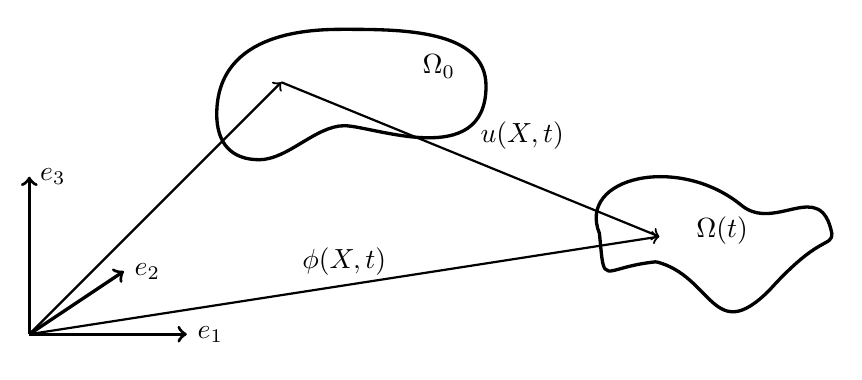
\begin{tikzpicture}[scale=0.8]
  %\draw[step=1.0,black,thin] (-3.,-1.) grid (3,4.);
  %\draw (-3,-1) -- (3,-1) -- (3,4) -- (-3,4) -- (-3,-1);
  \draw[very thick,->] (-5,-2.5) -- (-2.5,-2.5) node [right] {$\vect{e}_1$};
  \draw[very thick,->] (-5,-2.5) -- (-5,0.) node [right] {$\vect{e}_3$};
  \draw[very thick,->] (-5,-2.5) -- (-3.5,-1.5) node [right] {$\vect{e}_2$};
  \begin{scope}[scale=0.45]
    \draw[very thick] (-3,0.6) .. controls +(1,0) and +(-1,0) .. (0,1.8)  
    .. controls +(1,0) and +(0,-3) .. (5,3.2) 
    .. controls +(0,2) and +(2,0)  .. (0,5.2) 
    .. controls +(-1,0) and +(0,3) .. (-4.5,2.2) 
    .. controls +(0,-1) and +(-1,0).. (-3,0.6) ;
  \end{scope}
  \node at (1.5,1.75) {$\Omega_0$};
  %% Deformed body +2.
  \begin{scope}[scale=0.9]
    \draw[very thick] (0.+0.5+5.,0-1.5) ..controls (1.+0.5+5.,-0.25-1.5) and (1.+0.5+5.,-1.5-1.5) .. (2.+0.5+5.,-0.5-1.5) ..controls (2.9+0.5+5.,0.5-1.5) and (3.1+0.5+5.,0.25-1.5) .. (3.1+0.5+5.,0.5-1.5) ..controls (2.9+0.5+5.,1.5-1.5) and (2.1+0.5+5.,.5-1.5) .. (1.5+0.5+5.,1.-1.5) ..controls (0.4+0.5+5.,1.9-1.5) and (-1.4+0.5+5.,1.5-1.5) .. (-1.+0.5+5.,0.5-1.5)..controls (-0.4+0.+5.,-0.-2.) and (-1+0.5+5.,0.4-2.) .. (0+0.5+5.,0-1.5);
  \end{scope}
  \node at (6.,-0.85) {$\Omega(t)$};
  \draw[->,thick] (-5,-2.5) -- (-1.,1.5) node [midway,left] {$\X$};
  \draw[->,thick] (-5,-2.5) -- (5.,-0.95) node [midway,above] {$\vect{\phi}(\vect{X},t)$};
  \draw[->,thick] (-1.,1.5) -- (5.,-0.95) node [midway,above right] {$\vect{u}(\vect{X},t)$};
\end{tikzpicture}

%%% Local Variables:
%%% mode: latex
%%% TeX-master: "../../mainManuscript"
%%% End:
  \caption{Deformation of a solid body between a reference state $\Omega_0$ to a subsequent state $\Omega_t$.}
  \label{fig:deformationFunction}
\end{figure}

In the reference configuration, every material particle is located by their position vectors: $\vect{X}=X_\alpha \vect{e}_\alpha$, where $X_\alpha$ denotes the \textit{Lagrangian coordinates} and $\vect{e}_\alpha$ the basis vectors. At a subsequent time $t$, the particle initially located at $\vect{X}$ may have moved and its current location is given by the smooth mapping $\vect{\phi}(\vect{X},t)=\phi_i(\vect{X},t)\vect{e}_i$. Thus, the mapping $\vect{\phi}$ provides the paths of every particle of the solid during the deformation. In the lagrangian coordinates system, every particles are tracked during the deformation while the \textit{Eulerian coordinates}, denoted by $\vect{x}=x_i\vect{e}_i$, correspond to a \textit{spatial description}.
Note that in the above definitions Greek indices are used for quantities evaluated in the reference configuration whereas Latin ones refer to quantities defined in the current configuration. 

The \textit{displacement} and \textit{velocity} vectors of a particle between the reference and the current configuration are respectively:
\begin{align}
    &\vect{u}(\vect{X},t)=\vect{\phi}(\vect{X},t) - \vect{X} \qquad \forall\:\: \vect{X},t \in \Omega_0\times \tau  \label{eq:displacement}\\
    &\vect{v}(\vect{X},t)=\drond{\vect{\phi}}{t}(\vect{X},t) = \vect{\dot{\phi}}(\vect{X},t) \qquad  \forall\: \: \vect{X},t \in \Omega_0\times \tau  \label{eq:velocity}
\end{align}
where the superposed dot denotes the material time derivative. Then, the second-order two-point \textit{deformation gradient} tensor is defined as:
\begin{equation}
  \label{eq:F_phi}
    \tens{F}=\nablat_0 \vect{\phi} (\vect{X},t)
\end{equation}
where $\nablat_0 (\bullet)$ refers to the gradient operator on the reference configuration. This tensor can also be written by using equation \eqref{eq:displacement}:
\begin{equation}
  \tens{F}= \nablat_0 \vect{u}(\vect{X},t) + \tens{I} \label{eq:F_displacement}
\end{equation}
with $\tens{I}$, the second-order identity tensor. The deformation gradient tensor characterizes the variations of lengths, areas and volumes. Indeed, the infinitesimal vector, oriented surface and volume elements respectively denoted by $\vect{dX},\vect{dS}$ and $dV$ and defined in the reference configuration transorm respectively to:
\begin{equation}
  \label{eq:transport_equations}
  \begin{aligned}
    & dx_i=F_{i\alpha}dX_\alpha \\
    & ds_i=J F_{\alpha i}^{-1}dS_{\alpha} \\
    & dv=JdV 
  \end{aligned}
\end{equation}
in the current configuration. The transport equations \eqref{eq:transport_equations} involve the determinant of the deformation gradient $J=\det(\tens{F})>0$, also called the \textit{Jacobian of the deformation}. The deformation gradient is a strain measure since it accounts for changes in lengths and angles (\textit{i.e. the change of shape of a body}). Other strain measures can be used such as the \textit{right Cauchy-Green} or the \textit{Green-Lagrange} tensors, respectively defined as:
\begin{equation*}
   \tens{C}=\tens{F}^T\tens{F} \quad ; \quad \tens{E}=\frac{1}{2}(\tens{C}-\tens{I})
\end{equation*}
where $\tens{I}$ is the second-order identity tensor. The Green-Lagrange tensor can also be written by means of equation \eqref{eq:F_displacement}:
\begin{equation*}
  \tens{E}=\frac{1}{2}(\nablat_0 \vect{u} + \nablat_0 \vect{u}^T + \nablat_0 \vect{u}\nablat_0 \vect{u}^T)
\end{equation*}
In particular, when the deformation involves displacement vectors such that $\norm{\nablat_0 \vect{u}} \ll 1$, the last (second-order) term of the previous definition can be neglected leading to:
\begin{equation}
  \label{eq:epsilon}
  \tens{E} \approx \frac{1}{2}(\nablat_0 \vect{u} + \nablat_0 \vect{u}^T) = \tens{\eps}
\end{equation}
with $\tens{\eps}$ the \textit{linearized strain tensor}, the symmetric part of the displacement gradient. Such deformations fall in the \textit{linearized geometrical framework} or \textit{infinitesimal theory} and are characterized by small strain but possibly large displacements. Furthermore, when the deformation leads to a displacement vector $\norm{\vect{u}} \ll 1$ reference and current configurations are considered as indentical. These situations correspond to the \textit{small strain} framework for which the reference and current configurations are considered as identical.

\subsection{Balance equations}
In this section a solid domain $\Omega(t)$ undergoing a deformation is still considered within the time interval $\tau = \[0,T\]$. According to the formulation adopted in \cite{Plohr}, time derivatives of geometrical relations \eqref{eq:F_phi} and \eqref{eq:epsilon} combined to the definition of the velocity field \eqref{eq:velocity} yields kinematic conservations laws. Those conservation laws reads respectively:
\begin{align}
  & \tens{\dot{F}} - \nablat_0\vect{v} = \tens{0} \label{eq:HE_kinematic}\\
  & \tens{\dot{\eps}} - \nablat^s\vect{v} = \tens{0} \label{eq:HPP_kinematic}
\end{align}
where $\nablat^s$ denotes the symmetric gradient operator.

Then, we consider the conservation of mass in the continuum during the deformation in integral form:
\begin{equation*}
  \int_\Omega \rho d\Omega = \int_{\Omega_0} \rho_0 d\Omega \qquad \forall \: t \in  \tau
\end{equation*}
which, with the third transport formula reads:
\begin{equation}
  \label{eq:mass_conservation_law}
  \int_{\Omega_0} \(J\rho - \rho_0\) d\Omega = 0
\end{equation}
Leading to the first balance equation, namely the local conservation of mass:
\begin{equation}
  \label{eq:mass_balance}
  \rho = \frac{\rho_0}{J} \qquad \forall \: \vect{X},t \: \in \Omega_0\times \tau
\end{equation}
In particular, the linearised geometrical framework automatically satisfies this relation since current and reference configurations are the same (\textit{i.e.} $\rho=\rho_0 \: \forall t\in\tau$).

We now move on to the equilibrium between acceleration effects, namely \textit{intertia}, and external forces undergone by a solid $\Omega$. This conservation law corresponds to \textit{Newton's second law}:
\begin{equation*}
  \int_\Omega \rho \vect{\dot{v}} d\Omega = \int_{\partial \Omega} \vect{t} dS + \int_{\Omega} \rho\vect{b}d\Omega \qquad \forall \: t \in  \tau
\end{equation*}
where $\vect{t}$ denotes surface forces and $vect{b}$ volume forces in the current configuration. We then introduce the symmetric second-order \textit{Cauchy stress tensor} $\tens{\sigma}$ by using Cauchy's theorem $\vect{t}=\tens{\sigma}\cdot \vect{n}$ where $\vect{n}$ is the outwerd normal vector to the surface element $dS$. 

For further developments, the divergence theorem is required:
\begin{equation}
  \label{eq:Ostrogradski_th}
  \int_{\partial \Omega} (\bullet)\cdot \vect{dS}=\int_\Omega \nablav \cdot (\bullet) \: d\Omega
\end{equation}
where $\nablav \cdot (\bullet)$ denotes the divergence operator on the current configuration. Introduction of the previous formula in the second law of Newton leads to:
\begin{equation}
  \label{eq:Linear_momentum_conservation_eulerian}
  \int_{\Omega} \( \rho \vect{\dot{v}} - \nablav \cdot \tens{\sigma} -  \rho\vect{b} \) d\Omega = \vect{0} \qquad \forall \:t \in  \tau
\end{equation}
Conservation law \eqref{eq:Linear_momentum_conservation_eulerian} can be mapped to the reference configuration by using the transport formula of volume elements and the mass balance equation \eqref{eq:mass_balance}, thus yielding:
\begin{equation}
  \label{eq:Linear_momentum_conservation}
  \int_{\Omega_0} \( \rho_0 \vect{\dot{v}} - J \nablav \cdot \tens{\sigma} -  \rho_0\vect{b} \) d\Omega = \vect{0} \qquad \forall \: t \in\tau
\end{equation}
In equation \eqref{eq:Linear_momentum_conservation}, the divergence operator on the current configuration can be transported to the reference one by means of the \textit{Piola transform}:
\begin{definition}
  The Piola-Kirchhoff tranform $\tens{T}^P$ of a second-order tensor $\tens{T}$ is defined as:
  \begin{equation*}
    \tens{T}^P=J\tens{T}\cdot\tens{F}^{-1}
  \end{equation*}
  and satisfies:
  \begin{equation*}
    \nablav_0\cdot \tens{T}^P = J \nablav \cdot \tens{T}
  \end{equation*}
  where $\nablav_0\cdot (\bullet)$ is the divergence operator on the reference configuration.
\end{definition}
Another stress measure that corresponds to the Piola transform of Cauchy stress tensor is thus introduced, the \textit{first Piola-Kirchhoff stress tensor (PK1)} $\tens{\Pi}=J\tens{\sigma}\cdot\tens{F}^{-1}$. Hence, the vanishing of the integrand in equation \eqref{eq:Linear_momentum_conservation} yields the balance equation of the \textit{lagrangian linear momentum}:
\begin{equation}
  \label{eq:Lagrangian_linear_momentum}
  \rho_0 \vect{\dot{v}} - \nablav_0 \cdot \tens{\Pi} = \rho_0 \vect{b} \qquad \forall \: \: \vect{X},t \in \Omega_0 \times \tau 
\end{equation}
When considering deformations within the small strain framework the balance equation of linear momentum can be deduced from equation \eqref{eq:Linear_momentum_conservation_eulerian}, leading to:
\begin{equation}
  \label{eq:HPP_linear_momentum}
  \rho_0 \vect{\dot{v}} - \nablav \cdot \tens{\sigma} = \rho_0 \vect{b}  \qquad \forall \: \: \vect{x},t \in \Omega \times \tau 
\end{equation}

We complete the set of balance laws by considering the conservation of the energy of a system, also known as the \textit{first law of thermodynamics}. This law relates a balance between the rates of change of \textit{kinetic} and \textit{internal} energies, the power of external forces and the amount of heat entering the system as \textit{volume} or \textit{surface heat sources}.
\begin{equation*}
  \ddroit{}{t}\int_{\Omega} \(\frac{1}{2}\rho \vect{v}\cdot\vect{v} + \rho e\) d\Omega = \int_{\partial \Omega} \(\tens{\sigma}\cdot\vect{n}\)\cdot\vect{v} \: dS + \int_{\Omega} \rho\vect{b}\cdot\vect{v} \: d\Omega + \int_{\Omega} \rho r \:d\Omega - \int_{\partial \Omega} \vect{q}\cdot\vect{n} \: dS \qquad \forall \: t \in  \tau 
\end{equation*}
where $\vect{q}$ is the outward heat flux vector and $r$ is a volume heat source. By using the divergence theorem \eqref{eq:Ostrogradski_th}, the previous equation reads:
\begin{equation*}
\ddroit{}{t}\int_{\Omega} \(\frac{1}{2}\rho \vect{v}\cdot\vect{v} + \rho e\) d\Omega = \int_{\Omega} \(\nablav\cdot(\tens{\sigma}\cdot\vect{v}) +  \rho\vect{b}\cdot\vect{v} \) d\Omega + \int_{\Omega} \rho r \: d\Omega  - \int_{\partial \Omega} \vect{q}\cdot\vect{n} \: dS \qquad \forall \: t \in  \tau 
\end{equation*}
The transport of this relation on the reference configuration based on \eqref{eq:transport_equations} allows to introduce the time derivative of the left-hand side in the integral
\begin{equation*}
\int_{\Omega_0} \(\rho_0 \vect{\dot{v}} + \rho_0 \dot{e}\) d\Omega = \int_{\Omega_0} \(J\nablav\cdot(\tens{\sigma}\cdot\vect{v}) +  \rho_0\vect{b}\cdot\vect{v} \) d\Omega + \int_{\Omega_0} \rho_0 r \:d\Omega- \int_{\partial \Omega_0} J\vect{q}\cdot \tens{F}^{-1}\cdot\vect{n} \: dS \qquad \forall \: t \in  \tau 
\end{equation*}
Then, substitution of the linear momentum according to equation \eqref{eq:Lagrangian_linear_momentum} yields, after some algebra, the conservation law of internal energy:
\begin{equation}
  \label{eq:conservation_law_energy}
  \int_{\Omega_0} \rho_0 \dot{e} d\Omega = \int_{\Omega_0} \tens{\Pi}:\nablat_0\vect{v}\: d\Omega + \int_{\Omega_0} \(\rho_0r  - \nablav_0 \cdot \vect{Q}\) d\Omega \qquad \forall \: t \in  \tau 
\end{equation}
where $\vect{Q}=J\vect{q}\cdot \tens{F}^{-1}$ is the lagrangian heat flux vector. We thus deduce the balance equation of internal energy on the reference configuration:
\begin{equation}
  \label{eq:energy_balance}
  \rho_0 \dot{e} -  \tens{\Pi}:\nablat_0\vect{v}  + \nablav_0 \cdot \vect{Q}  = \rho_0 r \qquad \forall \: \: \vect{X},t \in \Omega_0 \times \tau 
\end{equation}
where $\nablat_0\vect{v} = \tens{\dot{F}}$. Finally, the small strain version of equation \eqref{eq:energy_balance} is: 
\begin{equation}
  \label{eq:energy_balance_euler}
  \rho_0 \dot{e} -  \tens{\sigma}:\nablat^{s} \vect{v}  + \nablav \cdot \vect{q}  = \rho_0 r \qquad \forall \: \: \vect{x},t \in \Omega \times \tau 
\end{equation}
in which $\nablat^{s} (\bullet)$ denotes the symmetric part of the gradient, in particular: $\nablat^s \vect{v} = \tens{\dot{\eps}}$. Stress measures are conjugate to strain measures through the power. In what follows, stress and strain may respectively be refered to as \textit{thermodynamic forces} and \textit{internal variables} according to the thermodynamics framework. The former obey a \textit{state equation} while the latter describe the evolution of the thermodynamic system. 
\subsection{Constitutive equations -- Thermodynamics}
The closure of a problem is given by the constitutive equations (\textit{i.e state laws}) for the stress. Once and for all, we consider here constitutive models within the \textit{Generalized Standard Materials} (GSM) framework \cite{GSM}.

\subsubsection*{The general (hyper)elasticity formulation}
First, the \textit{Clausius-Duhem} inequality resulting from combination of first and second laws of thermodynamics, reads: 
\begin{equation}
  \label{eq:Clausius-Duhem}
  \underbrace{\phantom{\frac{1}{\theta}} \tens{\Pi}:\tens{\dot{F}} + \rho_0 \(\theta \dot{\eta} -\dot{e}\)}_{\Dscr^{int}} \:-\:  \underbrace{\frac{1}{\theta} \vect{q} \cdot \nablav_0 \theta}_{-\Dscr^{th}} \geq 0  \qquad \forall \: \: \vect{X},t \in \Omega_0 \times \tau 
\end{equation}
where $\Dscr^{int}$ and $\Dscr^{th}$ are respectively the specific mechanical and thermal dissipations. Equation \eqref{eq:Clausius-Duhem} results in vanishing dissipations for \textit{reversible} processes and in a strict inequality for \textit{irreversible} ones. Furthermore, a widely used assumption consists in considering that the mechanical and thermal dissipations simultaneously satisfy non-negativeness. Note that the \textit{Fourier's law} of conduction is based on the non-negativeness of the thermal dissipation and leads to the following definition of the heat flux vector in order to ensure the positivity of the thermal dissipation:
\begin{equation*}
  \label{eq:Fourier_law}
  \vect{q}=-\tens{k}\cdot\nablav_0 \theta
\end{equation*}


The internal energy density is a function of strain, \textit{entropy} $\eta$ and additional state variables $\Vc_p, \: (1\leq p \leq N)$ describing irreversible processes. Recall that calligraphic symbols denote column array. It is more convenient to use its \textit{Legendre transform}, the \textit{Helmholtz free energy density potential} $\psi\(\tens{F},\theta,\Vcb\)=e\(\tens{F},\eta,\Vcb\)-\theta \eta$ where $\theta$ is the temperature. The free energy density is supposed \textit{objective} or \textit{frame indifferent} \cite[p.255]{Simo}, concave with respect to temperature and convex with respect to other variables. The mechanical dissipation can then be rewritten as:
\begin{equation*}
  \Dscr^{int} = \tens{\Pi}:\tens{\dot{F}} - \rho_0 \(\dot{\psi} +\eta \dot{\theta}\) 
\end{equation*}
The time derivative of Helmholtz free energy density:
\begin{equation}
  \label{eq:derivative_psi}
  \dot{\psi} = \drond{\psi}{\tens{F}}:\tens{\dot{F}} + \drond{\psi}{\theta}\dot{\theta} + \drond{\psi}{\Vcb}\dot{\Vcb}
\end{equation}
can be introduced within the mechanical dissipation so that one gets:
\begin{equation}
  \label{eq:Dint_psi_factor}
  \Dscr^{int} = \(\tens{\Pi}- \rho_0 \drond{\psi}{\tens{F}} \):\tens{\dot{F}} - \rho_0 \(\drond{\psi}{\theta} +\eta\) \dot{\theta}  - \rho_0\drond{\psi}{\Vcb}\dot{\Vcb} 
\end{equation}


Since the mechanical dissipation must be non-negative regardless of the nature of the deformation, it must in particular vanish for a reversible isothermal process (\textit{i.e. $\theta=const$}) for which every additional internal variables are constant. With these considerations, we are left with the relation:
\begin{equation*}
  \( \tens{\Pi} - \rho_0\drond{\psi}{\tens{F}} \): \tens{\dot{F}} = 0
\end{equation*}
holding regardless of the deformation, and hence:
\begin{equation}
  \label{eq:PK1_definition}
  \rho_0\drond{\psi}{\tens{F}} = \tens{\Pi}
\end{equation}
A material is said \textit{hyperelastic} if there exist a \textit{stored energy function} $\rho_0\psi$ from which can be derived the first Piola-Kirchhoff stress tensor \cite[p.8]{Foundation_of_elasticity}. The time derivative of this relation leads to:
\begin{equation}
  \label{eq:HE_tangent}
  \tens{\dot{\Pi}} = \rho_0\ddrond{\psi}{\tens{F}}{\tens{F}}:\tens{\dot{F}} = \Hbb:\tens{\dot{F}} 
\end{equation}
where $\Hbb$ is the $4$th order \textit{tangent modulus} tensor. Equivalently we have for linear elasticity:
\begin{equation}
  \label{eq:Cauchy_definition}
  \rho_0 \drond{\psi}{\tens{\eps}} = \tens{\sigma}
\end{equation}
and:
\begin{equation}
  \label{eq:HPP_tangent}
  \tens{\dot{\sigma}} = \rho_0\ddrond{\psi}{\tens{\eps}}{\tens{\eps}}:\tens{\dot{\eps}} = \Cbb:\tens{\dot{\eps}} 
\end{equation}
In equation \eqref{eq:HPP_tangent}, $\Cbb$ is the $4$th order \textit{elastic stiffness} tensor which has major and minor symmetries. For isotropic elasticity, $C_{ijkl}=\lambda \delta_{ij}\delta_{kl} + \mu \(\delta_{ik}\delta_{jl}+\delta_{il}\delta_{jk}\)$ yields \textit{Hook's law} with $(\lambda,\mu)$ are Lamé parameters.

Similar considerations lead to the state laws for entropy and for additional thermodynamic forces :
\begin{equation}
  \label{eq:thermodynamic_forces}
  \drond{\psi}{\theta} = - \eta \quad ; \quad \rho_0\drond{\psi}{\Vcb}=\Acb
\end{equation}
where $\Acb$ are thermodynamic forces associated to internal variables $\Vcb$.
In what follows, we shall consider hyperelastic or linear elastic deformations that do not involve irreversible processes (\textit{e.g. damage or thermal softening}). Hence, additional internal variables and associated thermodynamic forces are not activated in such situations. However, the cases of \textit{elastoplasticity} and \textit{elasto-viscoplasticity}, involving such variables and forces, will be considered in the linearized geometrical framework.

\begin{remark}
  \label{rq:isothermal_deformation}
  Temperature has been introduced as an internal variable and requires the introduction of the heat equation for the closure of the system:
  \begin{equation*}
    \rho_0 C \dot{\theta} = \rho_0 r - \nablav_0 \cdot \vect{Q} - \rho_0 \drond{\psi}{\Vcb}\dot{\Vcb} + \theta \(\drond{\tens{\Pi}}{\theta}:\tens{\dot{F}} - \drond{\Acb}{\theta}\dot{\Vcb} \)
  \end{equation*}
  Nevertheless, we will restrict our attention in the following to isothermal deformation so that temperature can be omitted and internal energy balance equation \eqref{eq:energy_balance} or \eqref{eq:energy_balance_euler} is automatically satisfied. Indeed, for isothermal processes the heat equation leads to:
  \begin{equation*}
    \rho_0 r - \nablav_0 \cdot \vect{Q} = \rho_0 \drond{\psi}{\Vcb}\dot{\Vcb}
  \end{equation*}
  which, once introduced in the energy balance \eqref{eq:energy_balance} yields:
  \begin{equation*}
    \rho_0 \dot{e} - \tens{\Pi}:\tens{\dot{F}} = \rho_0 \drond{\psi}{\Vcb}\dot{\Vcb}
  \end{equation*}
  By using the free energy density time derivative \eqref{eq:derivative_psi} and noting that $\eta=-\drond{\psi}{\theta} =0$, we get that each side of the previous equation vanishes.
\end{remark}


\subsubsection*{History-dependent models in small strain}
While elasticity does not involve dissipation, plasticity is characterized by irreversible strain and hardening variables $\Vcb$ that account for the loading history undergone by every material particles. Within the linearized geometrical framework, the infinitesimal strain tensor $\tens{\eps}$ is assume to be additively decomposed into an elastic and a plastic part:
\begin{equation}
  \label{eq:additive_plast}
  \tens{\eps} = \tens{\eps}^e + \tens{\eps}^p
\end{equation}
such that the mechanical dissipation only involve the plastic part:
\begin{equation}
  \label{eq:HPP_dissipation}
  \Dscr^{int}=\tens{\sigma}:\tens{\dot{\eps}}^p -\rho_0 \drond{\psi}{\Vcb}\dot{\Vcb} \geq 0
\end{equation}

A \textit{yield condition} is defined with the \textit{yield function} $f(\tens{\sigma},\Acb)$ so that that the elastic domain $\Ebb$ in stress space $(\tens{\sigma},\Acb)$ corresponds to:
\begin{equation}
  \label{eq:elastic_convex}
  \Ebb = \{ (\tens{\sigma},\Acb)\: | \: f(\tens{\sigma},\Acb) \leq 0\}
\end{equation}
According to the GSM framework \cite{GSM} we assume the existence of a dissipation pseudo-potential $\Phi(\tens{\sigma},\Vcb)$, convex with respect to thermodynamic forces and vanishing at the origin of the $(\tens{\sigma},\Vcb)$ space. This pseudo-potential enables the derivation of the plastic \textit{flow} and \textit{hardening} rules:
\begin{subequations}
  \begin{alignat}{2}
    \label{eq:flow_rule_plast}
     \tens{\dot{\eps}}^p&=&&\drond{\Phi}{f}\drond{f}{\tens{\sigma}}\\
    \label{eq:hardening_rule_plast}
     \dot{\Vcb}& = -&&\drond{\Phi}{f}\drond{f}{\Acb}
  \end{alignat}
\end{subequations}
where $\drond{\Phi}{f}=\dot{p}$ is the \textit{plastic multiplier}. We then distinguish two cases:
\begin{itemize}
\item \textbf{Rate-independent} plasticity is based on the assumption that admissible thermodynamic forces lie within the elastic domain \eqref{eq:elastic_convex}. The plastic multiplier is used as a Lagrange multiplier in order to ensure $f(\tens{\sigma},\Acb)\leq 0$ and must obey the \textit{K{\"u}hn-Tucker compatibility conditions}:
\begin{equation}
  \label{eq:Kuhn_Tucker}
  \dot{p} \geq 0 \quad ; \quad f \leq 0 \quad ; \quad \dot{p}f =0 
\end{equation}
The plastic multiplier, or the \textit{equivalent plastic strain rate} is determined by the \textit{consistency condition}:
\begin{equation}
  \label{eq:consistency_condition}
  \dot{f}=0
\end{equation}

% In analogy with the elastic law \eqref{eq:HPP_tangent}, rate-independent plastic evolutions are governed by the \textit{elastoplastic tangent modulus}:
% \begin{equation}
%   \label{eq:HPP_tangent_plasticity}
%   \tens{\dot{\sigma}}=\Cbb^{ep}:\tens{\dot{\eps}}
% \end{equation}

\item \textbf{Viscoplasticity} or \textbf{rate-dependent} plasticity can be seen as a regularization of rate-independent plasticity that relaxes the condition $f(\tens{\sigma},\Acb)\leq 0$ and thus leads to admissible thermodynamic forces outside the elastic domain \cite[p.58]{Simo}. Furthermore, the plastic fluxes $\tens{\dot{\eps}}^p, \dot{\Vcb}$ are completely determined by the knowlegde of the dissipation pseudo-potential. 
\end{itemize}
\subsubsection*{Examples of constitutive laws}
We now specify the above discussion to constitutive models that will be used in the following of the manuscript.

$\newline$
\textbf{The neo-Hookean hyperelastic model} is well-suited to describe rubber-like materials and is based on the polyconvex stored energy function:
\begin{equation}
  \label{eq:neo-hook_energy}
  \rho_0 \psi(J,\tens{F})= \frac{\kappa}{2}(J-1)^2 + \frac{\mu}{2}\[J^{-2/3} (\tens{F}:\tens{F})-3 \]
\end{equation}
where $\kappa$ is the bulk modulus and $\mu$ the Lam\'e shear modulus. We then introduce the \textit{tensor cross product} \cite{cross_tensor_product} of two second order two-point tensors $\tens{a}$ and $\tens{c}$, defined as:
\begin{equation}
  \label{eq:cross_tensor_product}
  \(\tens{a} \tens{\times} \tens{c}\)_{i\alpha}= \Ec_{ijk} \Ec_{\alpha \beta \gamma} a_{j\beta}b_{k\gamma}
\end{equation}
where $\Ec_{ijk}$ is the \textit{Levi-Civita} permutation symbol. By making use of this operator, the Jacobian $J$ can be written:
\begin{equation*}
  J=\frac{1}{6}\(\tens{F}\ttimes\tens{F}\):\tens{F}
\end{equation*}
or equivalently 
\begin{equation*}
  J=\frac{1}{3}\tens{H}:\tens{F}
\end{equation*}
in which $\tens{H}=\frac{1}{3}\tens{F}\ttimes\tens{F}=J\tens{F}^{-T}$ is the \textit{adjoint tensor} of the deformation gradient. Note that by using the tensor cross product operator, one can easily show that $\drond{J}{\tens{F}}=\tens{H}$. With these definitions, the derivative of the stored energy function \eqref{eq:neo-hook_energy} with respect to the deformation gradient can be computed so that the PK1 tensor can be derived:
\begin{equation}
  \label{eq:PK1_neo-hook}
  \tens{\Pi} = \mu J^{-2/3} \[\tens{F}- \frac{1}{3}\(\tens{F}:\tens{F}\) \tens{F}^{-T}\] + \kappa \(J-1\)\tens{H}
\end{equation}

The acoustic tensor $A_{ij}=N_\alpha H_{i\alpha j\beta} N_\beta$ for the neo-Hookean hyperelastic model is \cite{Haider_FVM}:
\begin{equation}
  \label{eq:neo-hook_acoustic}
  \begin{split}
      \tens{A}=\[\frac{5}{9}\mu J^{-8/3}\(\tens{F}:\tens{F}\)   + \kappa \]&(\tens{H}\cdot\vect{N})\otimes\(\tens{H}\cdot\vect{N} \)  + \mu J^{-2/3} \tens{I}  \\ &-\frac{2}{3}\mu J^{-5/3}\[(\tens{H}\cdot\vect{N})\otimes\(\tens{F}\cdot\vect{N} \)	+  (\tens{F}\cdot\vect{N})\otimes\(\tens{H}\cdot\vect{N} \)\]
  \end{split}
\end{equation}
The polyconvexity of this model ensures the positive definiteness of the acoustic tensor \eqref{eq:neo-hook_acoustic} \cite{Kluth}.

$\newline$
\textbf{The Saint-Venant-Kirchhoff hyperelastic model} is an extension of linear elastic Hook's law to hyperelasticity with a stored energy function that takes the form:
\begin{equation}
  \label{eq:SVK_energy}
  \rho_0\psi=\frac{1}{8}\(\tens{F}^T\tens{F}- \tens{I}\):\Cbb:\(\tens{F}^T\tens{F}- \tens{I}\)
\end{equation}
where $\Cbb$ is the elasticity tensor. In a similar manner as for the neo-Hookean model, the expression of the PK1 tensor is:
\begin{equation}
  \label{eq:SVK_PK1}
  \tens{\Pi} = \frac{1}{2}\lambda \(\tens{F}:\tens{F}- 3\) \tens{F} + \mu\tens{F}\(\tens{F}^T\tens{F}- \tens{I}\)
\end{equation}
The tangent modulus is then obtained by deriving this stress tensor:
\begin{equation}
  \label{eq:SVK_tangent}
  \Hbb = \lambda \[\tens{F}\otimes\tens{F} + \frac{1}{2} (\tens{F}:\tens{F}- 3)\Ibb\]+ \mu\(\Abb- \Ibb \)
\end{equation}
with $A_{i\alpha j \beta}=F_{k\alpha}F_{k\beta}\delta_{ij} + F_{j\alpha}F_{i\beta} +F_{i\mu} F_{j\mu}\delta_{\alpha\beta}$ and the fourth order identity tensor $I_{i\alpha j \beta}=\delta_{ij}\delta_{\alpha \beta}$. The previous tangent modulus finally leads to the acoustic tensor:
\begin{equation}
  \label{eq:SVK_acoustic}
  \begin{split}
    \tens{A} = \lambda \[\vphantom{\frac{1}{2}} (\tens{F}\cdot\vect{N})\otimes(\tens{F}\cdot\vect{N}) \right.+ &\left.\frac{1}{2} (\tens{F}:\tens{F}- 3)\tens{I}\] \\
    + & \mu\[(\tens{F}\cdot\vect{N})\cdot(\tens{F}\cdot\vect{N})\tens{I} + (\tens{F}\cdot\vect{N})\otimes(\tens{F}\cdot\vect{N}) + \tens{F}\cdot\tens{F}^T- \tens{I} \]
  \end{split}
\end{equation}
Even though it is known that this model can lead to non-physical solutions for very large deformation, it will be used for a one-dimensional strain problem for it enables to easily develop an analytical solution.  


$\newline$
\textbf{The plastic $J_2$ flow theory}, generally used to model metals, involves a yield function $f$ based on the second invariant of Cauchy stress deviatoric part $J_2=\tens{s}:\tens{s}$, where $\tens{s}=\tens{\sigma}-\frac{1}{3}\tr \tens{\sigma}$.
By considering internal variables and associated forces as: $\{\Vcb,\Acb\}=\{\[\tens{\eps}^p,p\],\[\tens{s}-\tens{Y},-R(p)\]\}$, one defines the following Helmoltz free energy density:
%can describe \textit{isotropic} linear hardening by setting $\tens{Y}=\tens{0}$, and \textit{kinematic} linear hardening with $R(p)=0$.The Helmoltz free energy density here reads:
\begin{equation}
  \label{eq:EP_helmoltz}
  \rho \psi = \frac{1}{2}\tens{\eps}^e:\Cbb:\tens{\eps}^e + \frac{2}{3}C\tens{\eps}^p:\tens{\eps}^p + H(r)
\end{equation}
In this expression, $r$ is to be defined, $H''(r)$ is the \textit{isotropic hardening} modulus and $\tens{Y}$ describes the evolution of the elastic domain center in stress deviator space and is related to \textit{kinematic hardening}. Linear hardenings will be considered here by setting either $\tens{Y}=\tens{0}$ for isotropic or $R(r)=0$ for kinematic hardening. The definition of thermodynamic forces \eqref{eq:thermodynamic_forces} leads to:
\begin{subequations}
  \begin{alignat}{1}
    \label{eq:eta}
    \tens{Y}&=\frac{2}{3}C\tens{\eps}^p \\
    \label{eq:isotropic_hardening}
    R &=H'(r)
  \end{alignat}
\end{subequations}
Furthermore, the \textit{von-Mises yield surface} is defined as:
\begin{equation}
  \label{eq:von-Mises_yield}
  f\(\tens{\sigma},\Acb \)= \sqrt{\frac{3}{2}}\norm{\tens{s}-\tens{Y}} - \(R(r)+\sigma^y\) \equiv 0
\end{equation}
$\sigma^y$ being the traction yield stress. The specialization of flow rules \eqref{eq:flow_rule_plast},\eqref{eq:hardening_rule_plast} leads to:
\begin{subequations}
  \begin{alignat}{1}
    \label{eq:plastic_strain_rate}
    &\tens{\dot{\eps}}^p=\dot{p}\sqrt{\frac{3}{2}}\frac{\tens{s}-\tens{Y}}{\norm{\tens{s}-\tens{Y}}}=\dot{p}\:\sqrt{\frac{3}{2}}\tens{m} \\
    \label{eq:equiv_plastic_strain_rate}
    &\dot{r}=\dot{p}
  \end{alignat}
\end{subequations}
where $r$ is identified from \eqref{eq:equiv_plastic_strain_rate} as the equivalent plastic strain. Considering rate-independent plasticity and combining the elastic law $\tens{\dot{\sigma}}=\Cbb:\(\tens{\dot{\eps}}-\tens{\dot{\eps}}^p\)$ yields the following evolution law:
\begin{equation}
  \label{eq:p_evolution}
  \dot{p}=\sqrt{\frac{3}{2}}\frac{2\mu}{3\mu+\beta}\tens{m}:\tens{\dot{\eps}}
\end{equation}
where $\beta=C$ for kinematic hardening and $\beta=R'(p)$ for isotropic hardening. Finally, equations \eqref{eq:plastic_strain_rate} and \eqref{eq:p_evolution}can be sequencially introduced in the elastic law so that one gets \cite[eq (2.2.22)]{Simo}:
\begin{equation}
  \label{eq:elastoplastic_tangent}
  \tens{\dot{\sigma}}=\(\Cbb - \frac{6\mu^2}{3\mu +\beta}\tens{m}\otimes\tens{m} \):\tens{\dot{\eps}} = \Cbb^{ep}:\tens{\dot{\eps}}
\end{equation}
with $\Cbb^{ep}$ the \textit{elastoplastic tangent modulus}. Note that (positive) linear hardenings ensure the positive definiteness of the elastoplastic acoustic tensor $\tens{A}^{ep}=\tens{A}^{elast} -  \frac{6\mu^2}{3\mu +\beta} (\tens{m}\cdot{n})\otimes(\tens{m}\cdot{n})$.  

Viscoplasticity on the other hand, leads to an explicit definition of the equivalent plastic strain:
\begin{equation}
  \label{eq:EVP_creep_law}
  \dot{p}=\left\langle \frac{f}{\eta}\right\rangle^n
\end{equation}
where $\left\langle\bullet\right\rangle=\frac{\bullet + \abs{\bullet}}{2}$ is the positive part function, and $n$ and $\eta$ are parameters arrising from the relaxation of the condition $f\leq 0$. Hence, rate-dependent plasticity is driven by the elastic law in which $\tens{\dot{\eps}^p}$ is given by \eqref{eq:flow_rule_plast} and \eqref{eq:EVP_creep_law}. 

\subsection{The general formulation}
We now summarize the conservation and constitutive laws obtained previously. Recall that the deformations considered here are isothermal and that history-dependent materials will be taken into account within linearized geometrical framework only. 
\subsubsection*{Linear elasticity and elasto-viscoplasticity}
We first gather the governing equations of elasticity and elasto-viscoplasticity within the linearized geometrical framework namely, the elastic law \eqref{eq:HPP_tangent}, the balance equation of linear momentum \eqref{eq:HPP_linear_momentum} and the kinematic law \eqref{eq:HPP_kinematic} which are repeated here for convenience:
\begin{align*}
  & \rho_0 \vect{\dot{v}} - \nablav \cdot \tens{\sigma} = \rho_0 \vect{b} \\
  & \tens{\dot{\sigma}} - \Cbb :\(\tens{\dot{\eps}}-\tens{\dot{\eps}}^p\) =\tens{0}\\
  & \tens{\dot{\eps}}-\nablat^s \vect{v} =\tens{0} \quad \qquad \forall \: \: \vect{x},t \in \Omega \times \tau 
\end{align*}
Note that the gradient operator of a vector $\vect{a}$ can be rewritten as a divergence operator:
\begin{equation}
  \label{eq:grad_div}
  \nablat \vect{a} = \nablav \cdot \(\vect{a}\otimes\tens{I} \)
\end{equation}
Hence, introduction of kinematic laws in the linear momentum balance yields, by assuming a cartesian coordinates system, the following \textit{conservative form}:
\begin{equation}
  \label{eq:general_conservative}
  \Qcb_t + \sum_{i=1}^D \drond{\Fcb\cdot \vect{e}_i}{x_i} = \Scb
\end{equation}
where the vector of conserved quantities $\Qcb$, fluxes vectors $\Fcb\cdot \vect{e}_i$ and the source term $\Scb$ are:
\begin{equation}
  \label{eq:vectors_elasticity}
  \Qcb =\matrice{\vect{v} \\ \tens{\sigma}} \quad ; \quad \Fcb\cdot\vect{e}_i = \matrice{-\frac{1}{\rho_0}\tens{\sigma}\cdot\vect{e}_i\\-\Cbb:\frac{\vect{v}\otimes\vect{e}_i +\vect{e}_i \otimes\vect{v} }{2} } \quad ; \quad \Scb = \matrice{ \vect{b} \\ -\Cbb:\tens{\dot{\eps}}^p}
\end{equation}
The quasi-linear form of equation \eqref{eq:general_conservative} is written by using the chain rule:
\begin{equation}
  \label{eq:HPP_quasi-linear}
  \Qcb_t + \Absf^i \drond{\Qcb}{x_i} = \Scb
\end{equation}
where:
\begin{equation*}
  \Absf^i=\drond{\Fcb\cdot \vect{e}_i}{\Qcb}=-\matrice{\tens{0}^3 & \frac{1}{\rho_0}\tens{I}\otimes\vect{e}_i\\\Cbb\cdot\vect{e}_i & \tens{0}^4}
\end{equation*}
in which symmetries of the elastic stiffness tensor have been used and $\tens{0}^p$ is a $p$th order null tensor. Since the elastic stiffness tensor is constant, system \eqref{eq:HPP_quasi-linear} is linear for elasticity and semi or non-linear for elasto-viscoplasticity depending on the flow rule
\eqref{eq:flow_rule_plast}.
\subsubsection*{Elasto-plasticity and hyperelasticity}
The non-linear constitutive equations of elastoplasticity and hyperelasticity prevent the straightforward writing of a conservative form. Indeed, such a conservation laws system is instead based on kinematic laws \eqref{eq:HE_kinematic} or \eqref{eq:HPP_kinematic}.
% \begin{align}
%   & \tens{\dot{F}} - \nablat_0 \vect{v} = \tens{0} \\
%   & \tens{\dot{\eps}} - \nablat^s\vect{v}=\tens{0} 
% \end{align}
Then, a conservative form \eqref{eq:general_conservative} is also written:
\begin{equation}
  \label{eq:general_conservative2}
  \Wcb_t + \sum_{i=1}^D \drond{\Fcb\cdot \vect{e}_\alpha}{X_\alpha} = \Scb
\end{equation}
 with:
\begin{alignat}{4}
  \label{eq:vectors_hyperelasticity}
  &\Wcb =\matrice{\vect{v} \\ \tens{F}} \quad &&; \quad \Fcb\cdot\vect{e}_\alpha = \matrice{-\frac{1}{\rho_0}\tens{\Pi}\cdot\vect{e}_\alpha\\-\vect{v}\otimes\vect{e}_\alpha } \quad &&; \quad \Scb = \matrice{ \vect{b} \\ \tens{0}} \quad &&\text{ for hyperelasticity}\\
  &\label{eq:vectors_plasticity}
  \Wcb =\matrice{\vect{v} \\ \tens{\eps}} \quad &&; \quad \Fcb\cdot\vect{e}_i = \matrice{-\frac{1}{\rho_0}\tens{\sigma}\cdot\vect{e}_i\\-\frac{\vect{v}\otimes\vect{e}_i +\vect{e}_i \otimes\vect{v} }{2} } \quad &&; \quad \Scb = \matrice{ \vect{b} \\\tens{0}} \quad &&\text{ for elastoplasticity}
\end{alignat}

Quasi-linear form are then built by introducing an auxiliary vector $\Qcb$ and using the chain rule according to \cite{Trangenstein91}:
\begin{equation}
  \label{eq:quasi-linear_Trangenstein}
  \drond{\Qcb}{t} + \(\drond{\Wcb}{\Qcb}\)^{-1}\drond{\Fcb\cdot\vect{e}_\alpha}{\Qcb} \drond{\Qcb}{X_\alpha} = \(\drond{\Wcb}{\Qcb}\)^{-1}\Scb = \tilde{\Scb}
\end{equation}
with the auxiliary vectors for elastoplasticity and hyperelasticity respectively defined as:
\begin{equation}
  \label{eq:auxiliary_vectors}
  \Qcb=\matrice{\vect{v}\\\tens{\sigma}} \quad ; \quad \Qcb=\matrice{\vect{v}\\\tens{\Pi}}
\end{equation}

Denoting momentarily and generically the stress measures by $\tens{S}$ and the strain measures by $\tens{P}$ so that $\Wcb^T=\[\vect{v},\tens{P}\]$ and $\Qcb^T=\[\vect{v},\tens{S}\]$, the matrix $\drond{\Wcb}{\Qcb}$ and its inverse are:
\begin{equation*}
  \drond{\Wcb}{\Qcb}=\matrice{\tens{I} & \tens{0}^3 \\ \tens{0}^3  & \drond{\tens{P}}{\tens{S}}} \Rightarrow \(\drond{\Wcb}{\Qcb}\)^{-1}=\matrice{\tens{I} & \tens{0}^3 \\ \tens{0}^3  & \drond{\tens{S}}{\tens{P}}}
\end{equation*}
in which $\drond{\tens{S}}{\tens{P}}$ is the tangent modulus of the considered constitutive model. Moreover, the derivative of the flux vectors with respect to the auxiliary vector has two different expressions depending on the constitutive model due to the symmetric gradient used for the linearized geometrical framework. On gets for hyperelastic materials:
\begin{equation}
  \drond{\Fcb\cdot\vect{e}_\alpha}{\Qcb}=-\matrice{\tens{0}^2 & \frac{1}{\rho_0}\tens{I}\otimes\vect{e}_\alpha \\    \tens{I}\boxtimes \vect{e}_\alpha & \tens{0}^4}
\end{equation}
while elastoplasticity leads to:
\begin{equation}
  \drond{\Fcb\cdot\vect{e}_i}{\Qcb}=-\matrice{\tens{0}^2 & \frac{1}{\rho_0}\tens{I}\otimes\vect{e}_i \\  \frac{\tens{I}\boxtimes \vect{e}_i+\vect{e}_i\otimes\tens{I}}{2} & \tens{0}^4   }
\end{equation}
in which the operator $\tens{I}\boxtimes\vect{e}_i$ is the transpose on second and third indices of the classical tensor product: $\tens{I}\boxtimes\vect{e}_i=\delta_{jk} \vect{e}_j\otimes \vect{e}_i\otimes\vect{e}_k$.

Finally, the quasi-linear forms associated to hyperelastic problems and elastoplastic ones are respectively:
\begin{alignat}{2}
  & \Qcb_t + \Absf^\alpha \drond{\Qcb}{X_\alpha} = \tilde{\Scb} \qquad &&\text{with: }\Absf^\alpha = -\matrice{ \tens{0}^2 & \frac{1}{\rho_0}\tens{I}\otimes\vect{e}_\alpha \\ \Hbb\cdot\vect{e}_\alpha & \tens{0}^4} \label{eq:HE_quasilinear}\\
  & \Qcb_t + \Absf^i \drond{\Qcb}{x_i} = \tilde{\Scb} \qquad &&\text{with: }\Absf^i = -\matrice{\tens{0}^2 & \frac{1}{\rho_0}\tens{I}\otimes\vect{e}_i\\ \Cbb^{ep}\cdot \vect{e}_i & \tens{0}^4} \label{eq:EP_quasilinear}
\end{alignat}
where the symmetries of the elastic stiffness tensor have been used. Note that the dependence on $\Qcb$ of matrices $\Absf(\Qcb)$ has been omitted for simplicity

%%% Local Variables:
%%% mode: latex
%%% TeX-master: "../mainManuscript"
%%% End:



\section{Characteristic analysis}
\label{sec:characteristic_analysis}
The eigenspaces of conservation laws systems defined above will be now investigated. As we shall see, the characteristic structure of those problems may lead to different type of waves propagating within a medium. Finally, existing analytical solutions of one-dimensional problems \cite{Wang} will be reviewed and that of a one-dimensional problem involving a hyperelastic \textit{Saint-Venant-Kirchhoff} material will be developed in order to illustrate the identified wave structures.
\subsection{Characteristic structure of solutions}
For the sake of simplicity studies of finite deformation and linearized geometrical frameworks will be condensed in this part by using a generic stress measure $\tens{S}$ and vectors written in the reference configuration. Furthermore, instead of studying multi-dimensional conservation laws systems, we will focus without loss of generality on conservative forms \eqref{eq:general_conservative} projected on an arbitrary direction $\vect{N}=\[\vect{e}_1,\vect{e}_2,\vect{e}_3\]$ \cite[p.425-426]{Leveque}. In this direction, the quasi-linear forms determined above are rewritten as:
\begin{equation}
  \label{eq:normal_quasi}
  \Qcb_t + \Jbsf \drond{\Qcb}{X_N} = \Scb
\end{equation}
where $X_N=\vect{X}\cdot\vect{N}$ and the \textit{Jacobian matrix} $\Jbsf = \Absf^\alpha N_\alpha$ arise. Hence, the characteristic analysis of system \eqref{eq:normal_quasi} is equivalent to that of linear combinations of matrices $\Absf^\alpha$. With the previous developments, the Jacobian matrix reads:
\begin{equation}
  \label{eq:jacobian_generic}
  \Jbsf=-\matrice{\tens{0}^2 & \frac{1}{\rho_0}\tens{I}\otimes \vect{N} \\  \tilde{\Hbb}\cdot\vect{N} & \tens{0}^4 }
\end{equation}
in which $\tilde{\Hbb}$ is either the hyperelastic or elastoplastic tangent modulus, or the elastic stifness tensor depending on the case considered. For general three-dimensional case, the characteristic structure of the problem is given by the $12$ eigenvalues $\lambda_k$ and associated left eigenvectors $\Lcb^k$ of the Jacobian matrix:
\begin{equation}
  \label{eq:eigen_system}
  \vect{\Lc}^k\cdot \(\Jbsf - \lambda_k \Ibsf\) = \vect{0}
\end{equation}
where $\Ibsf$ is the identity matrix and $\vect{\Lc}^k= \[ \vect{v}^K \: , \: \tens{S}^K \]$, with $\tens{S}$ standing for the suitable stress mesure. Thus, for non-null eigenvalues one gets:
\begin{subequations}
  \begin{alignat}{1}
    \label{eq:eigen_left_stress}
    & -\tens{S}^k:\(\tilde{\Hbb}\cdot  \vect{N}\) - \lambda_k  \vect{v}^k =\vect{0} \\
    \label{eq:eigen_left_velo}
    & -\frac{1}{\rho_0}\vect{v}^k\otimes\vect{N} - \lambda_k \tens{S}^k = \tens{0}
  \end{alignat}
\end{subequations}
Substitution of $\tens{S}$ obtained from \eqref{eq:eigen_left_velo} in \eqref{eq:eigen_left_stress} leads to:
\begin{equation}
  \label{eq:acoustic_eigen}
 (\vect{v}^k\otimes\vect{N}):\(\tilde{\Hbb}\cdot  \vect{N}\) - \rho_0\lambda^2_k \vect{v}^k = \tens{0}
\end{equation}
System \eqref{eq:acoustic_eigen} is the \textit{acoustic tensor} $A_{ij}=N_\alpha \tilde{H}_{i\alpha j \beta}  N_\beta$ left eigensystem which, due to the symmetry of $\tens{A}$ is equivalent to the right eigensystem:
\begin{equation}
  \label{eq:acoustic_eigen_system_lambda}
  \(  N_\alpha \tilde{H}_{i\alpha j \beta}  N_\beta - \rho_0 \lambda_k^2 \delta_{ij} \) v_j^k =0
\end{equation}
or atlernatively with the eigenvalues $\omega_p$ and associated left eigenvectors of the acoustic tensor $\vect{l}^p\: \: (p=1,2,3)$:
\begin{equation}
  \label{eq:acoustic_eigen_system}
  \( \tens{A} - \omega_p \tens{I} \) \vect{l}^p = \vect{0}
\end{equation}
The condition for system \eqref{eq:normal_quasi} to be hyperbolic and have real eigenvalues and associated eigenvectors is thus ensured by the positive definiteness of the acoustic tensor, also known as the \textit{strong ellipticity} condition \cite{Foundation_of_elasticity}:
\begin{equation}
  \label{eq:strong_ellipticity}
  (\vect{m}\otimes \vect{N}): \tilde{\Hbb}: (\vect{m}\otimes \vect{N}) > 0 \quad \forall \vect{N},\vect{m} \in \Rbb^3 \: ; \: \vect{N},\vect{m} \ne \vect{0}
\end{equation}
If the condition holds, the acoustic tensor admits $3$ couples eigenvalues--eigenvectors $\{\omega_p,\vect{l}^p\}$ leading to $6$ couples $\{\lambda_k,\Lcb^k\}$ for the Jacobian matrix, the $6$ other eigenvalues being null \cite{Kluth}. The couples $\{\lambda_k,\Lcb^k\}$ are referred to as \textit{left characteristic fields}. The left eigenvectors associated to non-zero eigenvalues of the Jacobian matrix are obtained by using equation \eqref{eq:eigen_left_velo} so that the following $6$ eigenfields of quasi-linear form \eqref{eq:normal_quasi} can be defined:
\begin{equation}
  \label{eq:left_eigenfields}
    \left\lbrace \pm \sqrt{\frac{\omega_p}{\rho_0}} ; \quad \[\: \pm \rho_0\sqrt{\frac{\omega_p}{\rho_0}} \vect{l}^p , -\vect{l}^p\otimes \vect{N} \:\]  \right\rbrace ,\quad p=1,2,3
\end{equation}
At last, one has to find six independent left eigenvectors associated to the null eigenvalue of multiplicity $6$ by solving equation of \eqref{eq:eigen_left_stress} for the null eigenvalue:
\begin{equation}
  \label{eq:left_null_eigenvectors}
  \tens{S}^k:\(\tilde{\Hbb}\cdot  \vect{N}\) =\vect{0},\quad k=1,...,6
\end{equation}
Following the same procedure for right eigenvectors $\Rcb^k=\matrice{\vect{v}^k \\ \tens{S}^k}$, the Jacobian matrix right eigensystem reads:
\begin{subequations}
  \begin{alignat}{1}
    \label{eq:eigen_right_stress}
    & -\frac{1}{\rho_0}\tens{S}^k\cdot  \vect{N} - \lambda_k  \vect{v}^k =\vect{0} \\
    \label{eq:eigen_right_velo}
    & -\tilde{\Hbb}:\(\vect{v}^k\otimes\vect{N}\) - \lambda_k \tens{S}^k = \tens{0}
  \end{alignat}
\end{subequations}
which leads to the \textit{right eigen fields} associated to the non-null eigenvalues:
\begin{equation}
  \label{eq:right_eigenfields}
  \left\lbrace \pm \sqrt{\frac{\omega_p}{\rho_0}} ; \quad \[\: \pm \sqrt{\frac{\omega_p}{\rho_0}} \vect{l}^p , -\tilde{\Hbb}:\( \vect{l}^p\otimes \vect{N}\) \:\]  \right\rbrace ,\quad p=1,2,3
\end{equation}
In equation \eqref{eq:right_eigenfields}, $\{\omega_p,\vect{l}^p\}$ still denotes the eigenfields of the acoustic tensor. Moreover, the $6$ independent right eigenvectors associated to the zero eigenvalue required to complete the set of right characteristic fields must satisfy:
\begin{equation}
  \label{eq:right_null_eigenvectors}
  \tens{S}^k \cdot  \vect{N} =\vect{0},\quad k=1,...,6
\end{equation}

Note that since the right-hand side of equation \eqref{eq:normal_quasi} is not involved in the characteristic analysis, linear elasticity and elaso-viscoplasticity leads to the same characteristic structure.

The notions highlighted so far will be illustrated in the two following sections. The method of characteristics will lead to:
\begin{itemize}
\item[(i)] the well-known solution to the \textit{Riemann problem} on a elastic bar
\item[(ii)] the development of the solution the Riemann problem of a hyperelastic Saint-Venant-Kirchhoff medium undergoing a one-dimensional strain state
\end{itemize}
Furthermore, the \textit{Rankine-Hugoniot condition} for discontinuous waves, and the concept of \textit{shock} and \textit{simple} waves will be introduced.

\subsection{Linear problems}
A Riemann problem is a Cauchy problem composed of a hyperbolic system and piecewise constant initial data on both sides of an interface. In the arbitrary direction $\vect{N}=\[\vect{e}_1,\vect{e}_2,\vect{e}_3\]$, the Riemann problem reads:
\begin{equation}
  \label{eq:Riemann_problem}
  \begin{aligned}
  &\Qcb_t + \drond{\Fcb\cdot \vect{N}}{X_N} = \Scb, \\
  &\left\lbrace 
    \begin{aligned}
      & \Qcb(X_N,t=0) = \Qcb_L \quad \text{if } X_N< 0\\
      & \Qcb(X_N,t=0) = \Qcb_R \quad \text{if } X_N> 0
    \end{aligned}
    \right.
  \end{aligned}
\end{equation}

We consider a one-dimensional elastic medium of density $\rho$ undergoing one-dimensional stress and strain states within the infinitesimal framework: $\tens{\eps}=\eps\: \vect{e}_1\otimes \vect{e}_1$ ; $\tens{\sigma}=\sigma \:\vect{e}_1\otimes \vect{e}_1$, so that the bar hypothesis holds with $\vect{v}=v \vect{e}_1$. The Riemann problem consists then of problem \eqref{eq:Riemann_problem} for $\vect{N}=\vect{e}_1$.

Neglecting body forces without loss of generality and introducing \textit{Yound's modulus E} such that $\sigma = E\eps$, conserved quantities and flux vector are:
\begin{equation*}
  \Qcb = \matrice{v \\ \sigma} \quad ; \quad \Fcb = \matrice{-\frac{1}{\rho}\sigma \\ -Ev}
\end{equation*}
The eigenvalues and left eigenvectors of the corresponding Jacobian matrix are:
\begin{equation*}
  \lambda_{1,2} = \pm \sqrt{\frac{E}{\rho}}=\pm c \quad ; \quad \Lcb^p=\[\rho \lambda_p \:,\: -1\]
\end{equation*}
The system of ODE along the characteristic curves, given by characteristic equations \eqref{eq:PDEs_ODEs}, is:
\begin{equation}
  \label{eq:elast_charac_equation}
  \Lcb^p \cdot d\Qcb = 0 \quad \Rightarrow
  \left\lbrace
    \begin{aligned}
      & \rho c\: dv - d\sigma = 0\\
      -& \rho c\: dv - d\sigma = 0
    \end{aligned} \right.
\end{equation}
Consider now a point $P$ of the ($x,t$) plane at which we are looking for the solution. Applying the method of characteristic, we trace the two characteristic straight lines starting from the $x$-axis (along which $\Qcb$ is given) and passing through $P$ (see dashed lines in figure \ref{fig:elasticity_example}).  
\begin{figure}[h]
  \centering
  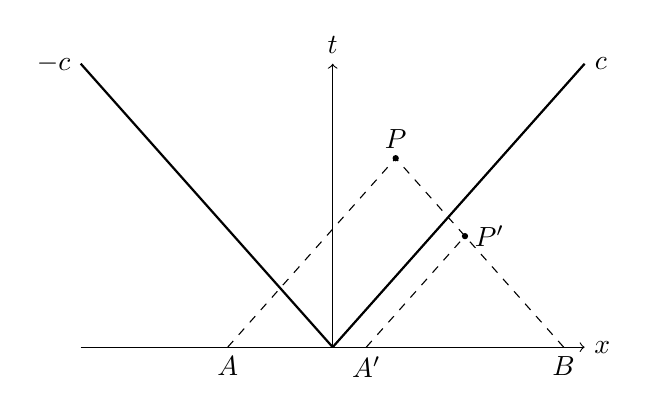
\begin{tikzpicture}[scale=0.8]
  \draw[->] (-4,0) -- (4.,0) node[right] {$x$};
  \draw[->] (0,0) -- (0,4.5) node[above] {$t$};
  \draw[thick] (0,0) -- (4.,4.5) node [right] {$c$};
  \draw[thick] (0,0) -- (-4.,4.5) node [left] {$-c$};
  \fill[black] (1.,3.) circle (0.05) node [above] {$P$};
  \draw[dashed] (1-8./3.,0.) node [below] {$A$}  -- (1.,3.);
  \draw[dashed] (1+8./3.,0.)node [below] {$B$}  -- (1.,3.);
  %% Intersection of positive solid line and negative dashed one
  %\fill[black] (0.5+12/9.,2.) circle (0.05) node [above] {$P'$};
  \fill[black] (2.10,1.762499) circle (0.05) node [right] {$P'$};
  \draw[dashed] (0.5333,0.) node [below] {$A'$}  -- (2.10,1.762499);
\end{tikzpicture}



%%% Local Variables:
%%% mode: latex
%%% TeX-master: "../../mainManuscript"
%%% End:

  \caption{Solution to Riemann problem \eqref{eq:Riemann_problem} for an elastic bar.}
  \label{fig:elasticity_example}
\end{figure}
Integration of characteristic equations \eqref{eq:elast_charac_equation} respectively along $AP$ and $BP$ yields:
\begin{equation}
  \label{eq:elastic_integral_curves}
  \left\lbrace
    \begin{aligned}
      & \rho c \(v_P - v_A \) - \(\sigma_P - \sigma_A \) = 0\\
      -& \rho c \(v_P - v_B \) - \(\sigma_P - \sigma_B \) = 0
    \end{aligned}
    \right.
\end{equation}
which solution is:
\begin{equation}
  \label{eq:elastic_solution_P}
  v_P = \frac{\sigma_B - \sigma_A}{2\rho c} + \frac{v_A+v_B}{2} \quad ; \quad \sigma_P = \rho c\frac{v_B - v_A}{2} + \frac{\sigma_A+\sigma_B}{2}
\end{equation}
On the other hand, the same procedure for point $P'$ leads to the solution:
\begin{equation}
  \label{eq:elastic_solution_Q}
  v_{P'} = \frac{\sigma_B - \sigma_{A'}}{2\rho c} + \frac{v_{A'}+v_B}{2} \quad ; \quad \sigma_{P'} = \rho c\frac{v_B - v_{A'}}{2} + \frac{\sigma_{A'}+\sigma_B}{2}
\end{equation}
With initial data given for the Riemann problem, it appears that $\Qcb_{A'}=\Qcb_{B}$ and hence, $\Qcb_{P'}=\Qcb_{R} \ne \Qcb_{P}$. Let's assume now that points $P$ and $P'$ are still on each side of the right characteristic straight line emanating from the origin but infinitely close to it. It is obvious that the previous results hold and that the a jump discontinuity propagates in the bar with speed $c$. Hence, we are left with the following condition across a discontinuous wave \cite{Toro} that generalizes to all linear Riemann problems:
\begin{definition}
Given a system of hyperbolic conservation laws $\Qcb_t + \Fcb(\Qcb)_x=\vect{0}$ and a discontinuous wave solution of speed $s_i$ associated to the $i$th characteristic field, the \textbf{Rankine-Hugoniot condition} reads:
\begin{equation}
  \label{eq:rankine-hugoniot}
  \saut{ \Fcb} = s_i \saut{ \Qcb}
\end{equation}
where $\saut{\bullet}$ denotes the jump operator across the discontinuity.  
\end{definition}


\textcolor{Red}{For non-linear discontinuities (shocks) the celerity $s_i$ is not known whereas in the linear case $s_i=\lambda_i$. (Then in the non-linear part, says that in that case the celerity of the shock is not known unlike for linear problems)}
\subsection{Non-linear problems}
We now consider a hyperelastic medium made of a Saint-Venant-Kirchhoff material, infinite in directions $\vect{e}_2$ and $\vect{e}_3$, and semi-infinite in direction $\vect{e}_1$ (\textit{i.e. $x_1 \in [0,+\infty[$}). This medium undergoes a load at $x_1=x=0$ in direction $\vect{e}_1$ so that the deformation gradient and the PK1 tensor are respectively:
\begin{align*}
  &\tens{F}=F\vect{e}_1\otimes\vect{e}_1 + \vect{e}_2\otimes\vect{e}_2 + \vect{e}_3\otimes\vect{e}_3 \\
  & \tens{\Pi}=\Pi_{11}\vect{e}_1\otimes\vect{e}_1 + \Pi_{22}\(\vect{e}_2\otimes\vect{e}_2 + \vect{e}_3\otimes\vect{e}_3 \)
\end{align*}
which corresponds to a plane wave solution. Once again, the Riemann problem considered is \eqref{eq:Riemann_problem} in which $\vect{N}=\vect{e}_1$ and:
\begin{equation*}
 \Qcb = \matrice{v \\ F} \quad ; \quad \Fcb = \matrice{-\frac{1}{\rho_0}\Pi_{11} \\ -v}
\end{equation*}
with neglected body forces. Since the tangent modulus and the acoustic tensor of Saint-Venant-Kirchhoff model \eqref{eq:SVK_tangent},\eqref{eq:SVK_acoustic} depend on the deformation gradient, the integration of characteristic equations \eqref{eq:PDEs_ODEs} is simpler with the quasi-linear form: $\Qcb_t + \drond{\Fcb}{\Qcb}\drond{\Qcb}{X_N}=\vect{0}$ which Jacobian matrix is:
\begin{equation}
  \label{eq:quasi_SVK}
  \Jbsf=\drond{\Fcb}{\Qcb}=-\matrice{0 & -\frac{H_{1111}}{\rho_0} \\ 1 & 0}
\end{equation}
The eigenvalues of this system are similar to that of the general case \eqref{eq:left_eigenfields} but the left eigenvectors are different and yield the following characteristic fields:
\begin{equation}
  \label{eq:SVK_charac_fields}
  \lambda_{1,2}=\pm \sqrt{\frac{\lambda+2\mu}{2\rho_0}\(3F^2-1\) } \quad ; \quad \Lcb^p=\[1\:,\:- \lambda_p \] \quad ; \quad \Rcb^p=\matrice{- \lambda_p \\1} 
\end{equation}
The non-linearity of the problem thus appears in characteristic speeds and eigenvectors.
\begin{definition} A characteristic field is said to be \textbf{genuinely non-linear} if
  \begin{equation}
    \label{eq:linearly-degenerate}
    \nablav_\Qc \lambda_i \cdot \Rcb^i \neq \vect{0},\quad \forall \Qcb \in \Rbb^m
  \end{equation}
\end{definition}
\begin{definition}
  A characteristic field is said to be \textbf{linearly degenerate} if it satisfies
  \begin{equation}
    \label{eq:linearly-degenerate}
    \nablav_\Qc \lambda_i \cdot \Rcb^i = \vect{0},\quad \forall \Qcb \in \Rbb^m
  \end{equation}
  where $\nablav_\Ucb (\bullet)$ is the gradient in the \textit{phase plane} $\(\Uc_1,...,\Uc_m \)$. In particular, linear systems for which eigenvalues are constant, admit only linearly degenerate characteristic fields.
\end{definition}

For the Saint-Venant-Kirchhoff material, equations \eqref{eq:SVK_charac_fields} lead to:
\begin{equation*}
  \nablav_\Qc \lambda_p = \matrice{0\\ \frac{3(\lambda+2\mu)F}{2\rho_0\lambda_p} } \quad \Rightarrow \nablav_\Qc \lambda_p \cdot \Rcb^p = \frac{3(\lambda+2\mu)F}{2\rho_0\lambda_p} 
\end{equation*}
with is not zero since $F>0$. The two characteristic fields are hence genuinely non-linear. However one must pay attention to the vanishing of characteristic speeds that can occur for $F=\frac{1}{\sqrt{3}}$. Indeed, we see that strain states for which $F \leq \frac{1}{\sqrt{3}}$ lead to a loss of hyperbolicity of the system for in such cases the eigenvalues of the Jacobian are non longer real.

\subsection{Integral curves}
\subsection{The Rankine-Hugoniot condition}


%%% Local Variables:
%%% mode: latex
%%% TeX-master: "../mainManuscript"
%%% End:



\section{Approximate Riemann solvers}
\label{sec:riemann_solvers}
It has been seen in the previous section that the complete solution of a Riemann problem in solid dynamics is possible for simple problems. However, such a solution may become complicated for multi-dimensional problems or for other non-linear problems. 
Numerical methods such as upwind or Godunov-based methods \cite{Leveque} require the solution of many Riemann problems within a discretized medium. When dealing with non-linear problems, the exact solution of those problems may increase drastically the computational cost, making the numerical scheme prohibitive. Moreover, numerical procedures often require only little information about the solution of Riemann problems and do not need the complete resolution. In that context, alternative procedures have been developed in order to take into account the characteristic structure of a hyperbolic system by computing an approximate solution of Riemann problems. Approximate Riemann solvers developed for Computational Fluid Dynamics allow to extract information for either flux functions (\textit{HLL, HLLC, Roe} and \textit{Osher} approximate Riemann solvers \cite{Trangenstein}, \cite{Toro}) or for vectors of conserved quantities (\textit{approximate--state Riemann solver} \cite[Ch.9]{Toro}, \cite[Ch.22]{Leveque}). Some of those have been applied to specific problems in solid mechanics problems such as the Osher approximate solver (see \cite{LEE_FVM} and \cite{Haider_FVM}) or the HLLC approximate solver (see \cite{Ortega_HLLD}) for hyperelasticity . We recall here the formulation of the approximate-state Riemann solver for solid mechanics. The approach is then applied to the non-linear problem of section \ref{sec:SVK_solution}.

\subsection{General ideas}
As in the previous section, we consider the Riemann problem in the space direction $\vect{N}$:
\begin{equation}
  \label{eq:RP_approx}
  \begin{aligned}
  &\Qcb_t + \Jbsf\(\Qcb\) \drond{\Qcb}{X_N} = \vect{0}, \\
  &\left\lbrace 
    \begin{aligned}
      & \Qcb(X_N,t=0) = \Qcb^L \quad \text{if } X_N< 0\\
      & \Qcb(X_N,t=0) = \Qcb^R \quad \text{if } X_N> 0
    \end{aligned}
    \right.
  \end{aligned}
\end{equation}
The approach for developing an approximate-state Riemann solver consists in linearizing the problem \eqref{eq:RP_approx} by approximating $\Jbsf$ in the vicinity of $\Qcb^L$ and $\Qcb^R$ by a constant matrix $\bar{\Jbsf}=\Jbsf\(\Qcb^L,\Qcb^R\)$ \cite[Ch.15]{Leveque}. Note that this approximation is valid for small jumps in initial data (\textit{i.e }$\Qcb^L\approx\Qcb^R$) and that $\bar{\Jbsf}$ must ensure hyperbolicity of the system, namely $\bar{\Jbsf}$ has real eigenvalues and a complete set of independent eigenvectors. The approximate matrix also satisfies the consistency condition:
\begin{equation}
  \label{eq:approx_constistency}
  \bar{\Jbsf}\(\Qcb,\Qcb\)=\Jbsf\(\Qcb\)
\end{equation}

Such a matrix can be defined by using the definition of right eigenvectors and characteristic speeds $\Jbsf \Rbsf = \Rbsf \Cbsf \Rightarrow \Jbsf = \Rbsf \Cbsf \Rbsf^{-1}$ in which left-going (\textit{resp. right-going}) characteristics and associated eigenvectors are assumed to depend on $\Qcb^L$ (\textit{resp. on} $\Qcb^R$) only. Namely, one writes:
\begin{align*}
  &\Rbsf = \matrice{\Rcb^1(\Qcb^L),\cdots,\Rcb^I(\Qcb^L),\Rcb^{I+1}(\Qcb^R),\cdots,\Rcb^m(\Qcb^R)} \\
  &\Cbsf=\matrice{c_1(\Qcb^L) & & & & & \\ & \cdots & & && \\ & &c_I(\Qcb^L) & & &\\ & & &c_{I+1}(\Qcb^R)& & \\ & & & &\cdots &\\ &&&&&c_m(\Qcb^R)} 
\end{align*}
where $c_I(\Qcb)$ and $m$ are the highest negative eigenvalue and the dimension of the Jacobian matrix. 

At last, the linearized Riemann problem thus written enables the determination of every state vectors $\Qcb(x,t)$ by following the procedure described in section \ref{subsec:charac_Linear_problems} for linear problems, recalled here for convenience for a system of dimension $m$:
\begin{equation}
  \label{eq:approx_RS}
  \begin{aligned}
    &  \Qcb^R-\Qcb^L=\sum_{i=1}^{m} \Rcb^i\delta^i \\
    &  \Qcb(x,t) =\Qcb^R -\sum_{i=I+1}^{m} \Rcb^i\delta^i \\
    &  \Qcb(x,t) =\Qcb^L+ \sum_{i=1}^{I} \Rcb^i\delta^i
  \end{aligned}
\end{equation}
where the point ($x,t$) lies in the region bounded by the $I$th and $I+1$th characteristics.

\begin{remark}
  Note that since one can define a complete set of independent eigenvectors of the Jacobian matrix, the matrix $\Rbsf$ is non-singular so that $\bar{\Jbsf}$ can be uniquely determined. Moreover, the linearization proposed amounts to considering a heterogeneous medium where $\Qcb^{L}$ and $\Qcb^R$ act as material parameters.
\end{remark}

\subsection{Application: Hyperelastic plane wave}
We finish this section with an illustration of the approximate Riemann solver by considering the plane wave problem in a Saint-Venant-Kirchhoff of section \ref{sec:SVK_solution}.
Recall that the eigenvalues and right eigenvectors matrices read for that problem:
\begin{equation}
  \label{eq:SVK_matrices}
  \Cbsf = \matrice{-c & 0 \\ 0 & c} \quad ; \quad \Rbsf = \matrice{c & -c\\ 1&1} \:,\quad c=\sqrt{\frac{\lambda + 2\mu}{2\rho_0}(3F^2-1)}
\end{equation}
Hence, the linearized problem is written with:
\begin{equation}
  \label{eq:SVK_matrices_linear}
  \Cbsf = \matrice{-c_L & 0 \\ 0 & c_R} \quad ; \quad \Rbsf = \matrice{c_L & -c_R\\ 1&1}
\end{equation}
In section \ref{subsec:charac_Linear_problems}, the expression of the wave strengths vector $\vect{\delta}$ has been established for general linear systems of dimension $2$ (see equation \eqref{eq:wave_strengths}):
\begin{equation}
  \vect{\delta}=\frac{1}{c_R+c_L}\matrice{c_R \Delta F +\Delta v\\ c_L \Delta F -\Delta v}
\end{equation}
leading to the solution $\Qcb $ between the two discontinuous waves:
\begin{equation}
  \label{eq:SVK_approx_solution}
  \Qcb  = \Qcb^L + \delta^1 \Rcb^1 = \matrice{v_L \\F_L} +\delta^1 \matrice{c_L \\1} \quad \text{or} \quad \Qcb  = \Qcb^R - \delta^2 \Rcb^2 = \matrice{v_R \\F_R} -\delta^2 \matrice{-c_R \\1}
\end{equation}
Substitutions of $\delta^{1,2}$ from second equations in first ones provide straight lines equations in the phase plane ($F,v$):
\begin{equation}
  \label{eq:approx_straight}
  v  = v_L + c_L(F -F_L) \quad ; \quad v  = v_R + c_R(F_R-F )
\end{equation}
\begin{figure}[h!]
  \centering
  {\definecolor{Purple}{RGB}{120,28,129}
\definecolor{Blue}{RGB}{63,96,174}
\definecolor{Duck}{RGB}{83,158,182}
\definecolor{Green}{RGB}{109,179,136}
\definecolor{Yellow}{RGB}{202,184,67}
\definecolor{Orange}{RGB}{231,133,50}
\definecolor{Red}{RGB}{217,33,32}
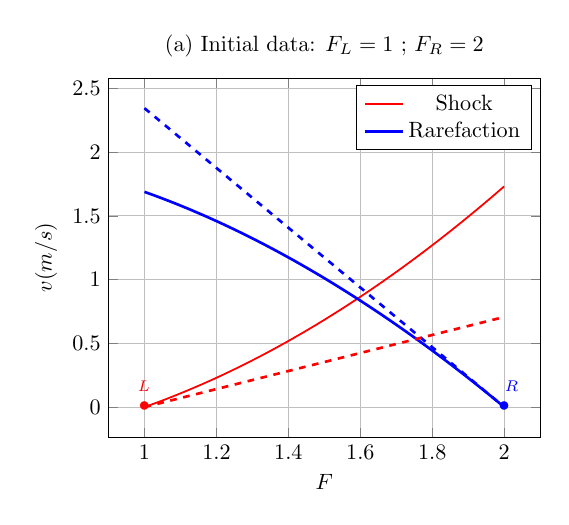
\begin{tikzpicture}[scale=0.8]
\begin{axis}[xlabel=$F$,ylabel=$v (m/s)$,ymajorgrids=true,xmajorgrids=true, title={(a) Initial data: $F_L=1$ ; $F_R=2$}]
  \addplot[Red,thick] coordinates {(1.0,0.0) (1.0196019601960196,0.019889905868838792) (1.0392039203920391,0.04035480171519238) (1.058805880588059,0.06139339246981025) (1.0784078407840785,0.08300445472552491) (1.098009800980098,0.1051868317293367) (1.1176117611761176,0.1279394287977403) (1.1372137213721372,0.1512612091133456) (1.1568156815681567,0.17515118986560513) (1.1764176417641765,0.19960843870261852) (1.196019601960196,0.2246320704646163) (1.2156215621562156,0.25022124417291264) (1.2352235223522352,0.2763751602509047) (1.2548254825482548,0.30309305795616337) (1.2744274427442743,0.330374213004825) (1.2940294029402941,0.3582179353714115) (1.3136313631363137,0.386623567248899) (1.3332333233323332,0.4155904811553686) (1.3528352835283528,0.445118078174895) (1.3724372437243724,0.47520578632153143) (1.3920392039203922,0.5058530590163028) (1.4116411641164117,0.5370593736680643) (1.4312431243124313,0.568824230349938) (1.4508450845084508,0.6011471505637854) (1.4704470447044704,0.6340276760858663) (1.4900490049004902,0.667465367887438) (1.5096509650965095,0.7014598051246006) (1.5292529252925293,0.7360105841921958) (1.5488548854885489,0.7711173178369951) (1.5684568456845684,0.8067796343258441) (1.5880588058805882,0.8429971766647708) (1.6076607660766076,0.8797696018654025) (1.6272627262726274,0.917096580255355) (1.646864686468647,0.9549777948294852) (1.6664666466646665,0.9934129406392047) (1.686068606860686,1.032401724217221) (1.7056705670567056,1.0719438630353144) (1.7252725272527254,1.1120390849929296) (1.7448744874487447,1.1526871279345328) (1.7644764476447645,1.1938877391938512) (1.784078407840784,1.2356406751632294) (1.8036803680368036,1.2779457008865038) (1.8232823282328234,1.320802589673878) (1.8428842884288428,1.3642111227374165) (1.8624862486248626,1.4081710888458763) (1.8820882088208821,1.4526822839976499) (1.9016901690169017,1.4977445111107466) (1.9212921292129215,1.543357579728744) (1.9408940894089408,1.5895213057417645) (1.9604960496049606,1.6362355111215798) (1.9800980098009802,1.6835000236699957) (1.9996999699969997,1.7313146767797576) };
  \addplot[Blue,very thick] coordinates {(1.0,1.6884673989302577) (1.0196019601960196,1.6685781823289632) (1.0392039203920391,1.648117983645035) (1.058805880588059,1.6270917763366024) (1.0784078407840785,1.6055041425368688) (1.098009800980098,1.5833593157699348) (1.1176117611761176,1.5606612177002648) (1.1372137213721372,1.5374134899261505) (1.1568156815681567,1.5136195216278194) (1.1764176417641765,1.48928247372591) (1.196019601960196,1.4644053000848238) (1.2156215621562156,1.4389907661996928) (1.2352235223522352,1.4130414657294894) (1.2548254825482548,1.3865598351776642) (1.2744274427442743,1.3595481669723095) (1.2940294029402941,1.3320086211576845) (1.3136313631363137,1.3039432358761032) (1.3332333233323332,1.2753539367920979) (1.3528352835283528,1.246242545588463) (1.3724372437243724,1.216610787645106) (1.3920392039203922,1.1864602989961286) (1.4116411641164117,1.1557926326474621) (1.4312431243124313,1.12460926432638) (1.4508450845084508,1.092911597724879) (1.4704470447044704,1.0607009692909792) (1.4900490049004902,1.0279786526152188) (1.5096509650965095,0.994745862453826) (1.5292529252925293,0.9610037584250569) (1.5488548854885489,0.9267534484108921) (1.5684568456845684,0.8919959916925568) (1.5880588058805882,0.8567324018451127) (1.6076607660766076,0.8209636494135533) (1.6272627262726274,0.7846906643903794) (1.646864686468647,0.7479143385125069) (1.6664666466646665,0.7106355273934435) (1.686068606860686,0.6728550525050632) (1.7056705670567056,0.6345737030218022) (1.7252725272527254,0.595792237538853) (1.7448744874487447,0.5565113856747698) (1.7644764476447645,0.5167318495678894) (1.784078407840784,0.47645430527509447) (1.8036803680368036,0.43567940408061234) (1.8232823282328234,0.3944077737218566) (1.8428842884288428,0.3526400195386741) (1.8624862486248626,0.31037672555176576) (1.8820882088208821,0.2676184554755838) (1.9016901690169017,0.22436575367049583) (1.9212921292129215,0.18061914603862234) (1.9408940894089408,0.13637914086738703) (1.9604960496049606,0.09164622962443836) (1.9800980098009802,0.04642088770736517) (1.9996999699969997,0.0007035751512764867) };
  \node at (axis cs:1,0) [Red] {$\bullet$};
  \node at (axis cs:2.,0) [Blue] {$\bullet$};
  \node at (axis cs:1,0) [anchor=south,Red] {$\Qcb^L$};
  \node at (axis cs:1.98,0) [above right,Blue] {$\Qcb^R$};
  \addplot[Blue,dashed,very thick,domain=1:2,samples=51,samples y=0]
    ({x},{0.-sqrt(0.5*(12.-1))*(x-2.)});
  \addplot[Red,dashed,very thick,domain=1:2,samples=51,samples y=0]
    ({x},{0.+sqrt(0.5*(2.-1))*(x-1.)});
  \legend{Shock,Rarefaction}
\end{axis}
\end{tikzpicture}
 \phantomsubcaption \label{subfig:SVK_Approx1}}
  {\definecolor{Red}{RGB}{217,33,32}
\definecolor{Blue}{RGB}{63,96,174}
\definecolor{Duck}{RGB}{83,158,182}
\definecolor{Green}{RGB}{109,179,136}
\definecolor{Yellow}{RGB}{202,184,67}
\definecolor{Orange}{RGB}{231,133,50}
\definecolor{Purple}{RGB}{120,28,129}
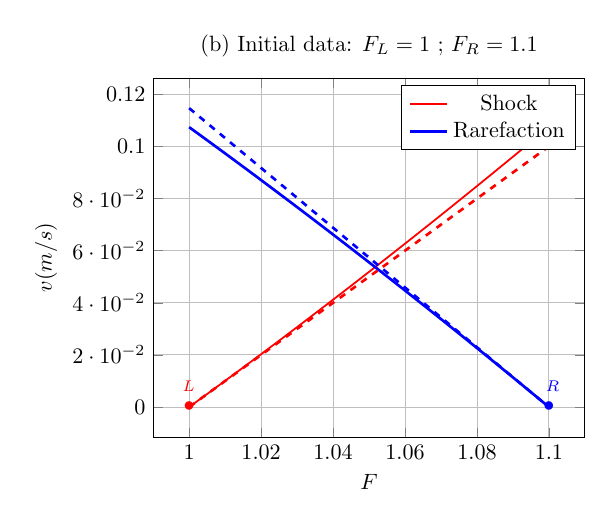
\begin{tikzpicture}[scale=0.8]
\begin{axis}[xlabel=$F$,ylabel=$v (m/s)$,ymajorgrids=true,xmajorgrids=true,title={(b) Initial data: $F_L=1$ ; $F_R=1.1$}]
\addplot[Red,thick] coordinates {(1.0,0.0) (1.001960196019602,0.0019630775609053948) (1.003920392039204,0.003931917267080632) (1.005880588058806,0.005906517718693416) (1.0078407840784078,0.007886877524091035) (1.00980098009801,0.009872995299740863) (1.0117611761176117,0.011864869670167599) (1.0137213721372138,0.01386249926789511) (1.0156815681568157,0.01586588273338493) (1.0176417641764177,0.01787501871497885) (1.0196019601960196,0.019889905868838792) (1.0215621562156216,0.02191054285889049) (1.0235223522352235,0.023936928356764118) (1.0254825482548255,0.025969061041739377) (1.0274427442744274,0.028006939600686957) (1.0294029402940295,0.030050562728014697) (1.0313631363136313,0.03209992912561001) (1.0333233323332334,0.034155037502787186) (1.0352835283528352,0.0362158865762309) (1.0372437243724373,0.03828247506994398) (1.0392039203920391,0.04035480171519238) (1.0411641164116412,0.04243286525045405) (1.0431243124312433,0.044516664421364406) (1.045084508450845,0.04660619798066565) (1.0470447044704472,0.048701464688155255) (1.049004900490049,0.050802463310633685) (1.050965096509651,0.05290919262185532) (1.052925292529253,0.055021651402476585) (1.054885488548855,0.05713983844000798) (1.0568456845684568,0.059263752528762766) (1.058805880588059,0.06139339246981025) (1.0607660766076608,0.06352875707092508) (1.0627262726272628,0.06566984514654145) (1.0646864686468647,0.06781665551770343) (1.0666466646664667,0.06996918701201955) (1.0686068606860686,0.07212743846361445) (1.0705670567056706,0.07429140871308419) (1.0725272527252725,0.07646109660744838) (1.0744874487448746,0.07863650100010654) (1.0764476447644764,0.08081762075079126) (1.0784078407840785,0.08300445472552491) (1.0803680368036805,0.08519700179657394) (1.0823282328232824,0.08739526084240548) (1.0842884288428845,0.08959923074764438) (1.0862486248624863,0.09180891040302837) (1.0882088208820884,0.09402429870536706) (1.0901690169016902,0.09624539455749745) (1.0921292129212923,0.09847219686824406) (1.0940894089408941,0.1007047045523746) (1.0960496049604962,0.10294291653056116) (1.098009800980098,0.1051868317293367) (1.0999699969997,0.10743644908105657) };
\addplot[Blue,very thick] coordinates {(1.0,0.1073874627707086) (1.001960196019602,0.10542438591418365) (1.003920392039204,0.10345555112494406) (1.005880588058806,0.10148096397787983) (1.0078407840784078,0.09950062999930058) (1.00980098009801,0.09751455466754301) (1.0117611761176117,0.09552274341357074) (1.0137213721372138,0.09352520162156171) (1.0156815681568157,0.0915219346294884) (1.0176417641764177,0.089512947729686) (1.0196019601960196,0.08749824616941433) (1.0215621562156216,0.08547783515140679) (1.0235223522352235,0.08345171983441528) (1.0254825482548255,0.08141990533374051) (1.0274427442744274,0.07938239672176006) (1.0294029402940295,0.07733919902844166) (1.0313631363136313,0.0752903172418546) (1.0333233323332334,0.07323575630866758) (1.0352835283528352,0.07117552113464229) (1.0372437243724373,0.06910961658511733) (1.0392039203920391,0.06703804748548585) (1.0411641164116412,0.06496081862166392) (1.0431243124312433,0.06287793474055453) (1.045084508450845,0.06078940055050131) (1.0470447044704472,0.05869522072173673) (1.049004900490049,0.056595399886824015) (1.050965096509651,0.05448994264109064) (1.052925292529253,0.05237885354305752) (1.054885488548855,0.05026213711485809) (1.0568456845684568,0.0481397978426566) (1.058805880588059,0.04601184017705303) (1.0607660766076608,0.04387826853348905) (1.0627262726272628,0.0417390872926421) (1.0646864686468647,0.0395943008008181) (1.0666466646664667,0.037443913370333926) (1.0686068606860686,0.03528792927989956) (1.0705670567056706,0.03312635277498877) (1.0725272527252725,0.03095918806820985) (1.0744874487448746,0.02878643933966615) (1.0764476447644764,0.026608110737315303) (1.0784078407840785,0.0244242063773199) (1.0803680368036805,0.022234730344396287) (1.0823282328232824,0.020039686692156212) (1.0842884288428845,0.017839079443443134) (1.0862486248624863,0.01563291259066641) (1.0882088208820884,0.013421190096127349) (1.0901690169016902,0.011203915892344065) (1.0921292129212923,0.008981093882367926) (1.0940894089408941,0.006752727940100287) (1.0960496049604962,0.00451882191059879) (1.098009800980098,0.0022793796103861676) (1.0999699969997,3.4404827748516585e-05) };
\node at (axis cs:1,0) [Red] {$\bullet$};
  \node at (axis cs:1.1,0) [Blue] {$\bullet$};
  \node at (axis cs:1,0) [anchor=south,Red] {$\Qcb^L$};
  \node at (axis cs:1.097,0) [above right,Blue] {$\Qcb^R$};
  \addplot[Red,dashed,very thick,domain=1:1.1,samples=51,samples y=0]
  ({x},{0.+sqrt(0.5*(3.-1))*(x-1.)});
  \addplot[Blue,dashed,very thick,domain=1:1.1,samples=51,samples y=0]
    ({x},{0.-sqrt(0.5*(3.*(1.1^2)-1))*(x-1.1)});
\legend{Shock,Rarefaction}
\end{axis}
\end{tikzpicture}
 \phantomsubcaption \label{subfig:SVK_Approx4}}
  \caption{Comparison of approximate (dashed lines) and exact (solid lines) solution for a one-dimensional strain problem in a Saint-Venant-Kirchhoff hyperelastic material}
  \label{fig:comparison_exact_approx}
\end{figure}
The intersection of those straight lines in the phase plane corresponds to the approximate solution. Figure \ref{fig:comparison_exact_approx} shows comparisons of approximate and exact solutions for various initial data, all leading to a $1$-shock--$2$-rarefaction exact solution. As expected, approximate and exact solutions are different and get closer for small initial discontinuities, falling in the linearization assumption $\Qcb^L\approx \Qcb^R$. As a consequence, in figures \ref{fig:comparison_exact_approx}\subref{subfig:SVK_Approx1} a big initial discontinuity is considered so that the approximation error is larger than that of figure \ref{fig:comparison_exact_approx}\subref{subfig:SVK_Approx4} for which initial data are based on a weak jump.


%%% Local Variables:
%%% mode: latex
%%% TeX-master: "../mainManuscript"
%%% End:





%%% Local Variables:
%%% mode: latex
%%% TeX-master: "../mainManuscript"
%%% End:
